%! Unidad 1 — Leyes fundamentales de la química (teoría, ejemplos resueltos, ejercicios por apartados y prácticas)
%! Fuente: Fuentes/Quimica/Unidad 1 (capturas 470-488 y solucionario). Texto reescrito; datos de los ejercicios cambiados y recalculados.
%! Masas atómicas usadas: H 1; C 12; N 14; O 16; Na 23; S 32; Cl 35,5; K 39; Cr 52; Fe 55,8; Cu 63,5; Ag 107,9; Pb 207,2.

\section*{Para empezar: de la alquimia a la química}
\addcontentsline{toc}{section}{Para empezar: de la alquimia a la química}

La química es heredera de la \textbf{alquimia}, una práctica que mezclaba conocimientos de metalurgia, medicina, farmacia
y filosofía y que buscaba, entre otras cosas, convertir los metales en oro. Los alquimistas descubrieron muchas sustancias y
técnicas de laboratorio, pero no tenían un método para comprobar sus ideas. Todo cambió con el \textbf{método científico}
del siglo \textsc{xvii}: \textbf{Robert Boyle} estudió el comportamiento de los gases y defendió que la química debía basarse en
experimentos; un siglo después, \textbf{Antoine Lavoisier} pesó con cuidado reactivos y productos y enunció la ley de
conservación de la masa; y a comienzos del siglo \textsc{xix}, \textbf{John Dalton} propuso la teoría atómica. En esta unidad
recorremos ese camino: las leyes que relacionan las masas y los volúmenes de las sustancias que reaccionan, la teoría que las
explica, el concepto de mol y el comportamiento de los gases.

\begin{remark}
    \textbf{Algunos hitos de la química.} Dominio del fuego y cerámica (hace unos \num{800000} años) ·
    embalsamamiento en Egipto (\num{3000} a.\,C.) · teoría atómica de Leucipo y Demócrito (440 a.\,C.) ·
    los cuatro elementos de Aristóteles (450 a.\,C.) · alquimia (desde el 300 a.\,C.) ·
    Paracelso y los primeros medicamentos (1530) · \emph{El químico escéptico} de Boyle (1661) ·
    Lavoisier, padre de la química moderna (1772) · teoría atómica de Dalton (1808) ·
    tabla periódica de Mendeléiev (1869) · Thomson descubre el electrón (1897) ·
    Baekeland fabrica la baquelita, el primer plástico sintético (1907) · Marie Curie y la radiactividad (1911) ·
    modelo atómico de Bohr (1913) · estructura del ADN (1953).
\end{remark}

%========================================================================================
\section{Recuerda de la ESO}\label{sec:ud1-eso}
%========================================================================================

\paragraph{La materia y sus propiedades.} \textbf{Materia} es todo lo que tiene masa y ocupa un lugar en el espacio. Sus
propiedades pueden ser \textbf{generales} (masa, volumen, temperatura), que no sirven para distinguir una sustancia de otra, o
\textbf{características} (densidad, punto de ebullición, dureza, color), que tienen un valor propio de cada sustancia. Otra
clasificación distingue las propiedades \textbf{extensivas}, que dependen de la cantidad de materia (masa, volumen), de las
\textbf{intensivas}, que no dependen de ella (temperatura, densidad).

Una \textbf{sustancia pura} tiene composición y propiedades fijas. Puede ser una \textbf{sustancia simple} o
\textbf{elemento} (oro, oxígeno, ozono), que no se descompone en otras más sencillas, o un \textbf{compuesto} (agua, dióxido
de carbono, cloruro de sodio), formado por varios elementos combinados en proporción fija. Las \textbf{mezclas} pueden ser
homogéneas o heterogéneas. En los \textbf{procesos físicos} no cambia la naturaleza de las sustancias (los cambios de estado,
por ejemplo); en los \textbf{procesos químicos} unas sustancias desaparecen y se forman otras nuevas (la combustión del papel).

\paragraph{Estados de agregación y teoría cinética.} Según la \textbf{teoría cinético-molecular}, la materia está formada por
partículas (átomos, moléculas o iones) en continuo movimiento. La intensidad de las fuerzas entre ellas explica los estados
(figura~\ref{fig:ud1-estados}): en los \textbf{sólidos} las fuerzas son intensas y las partículas solo vibran; en los
\textbf{líquidos} son moderadas y las partículas se deslizan unas sobre otras; en los \textbf{gases} son muy débiles y las
partículas se mueven libremente y ocupan todo el recipiente. La \textbf{temperatura} mide la energía cinética media de las
partículas, \(E_c = \frac{1}{2} m v^2\): cuanto mayor es, más deprisa se mueven.

\begin{figure}[H]
    \centering
    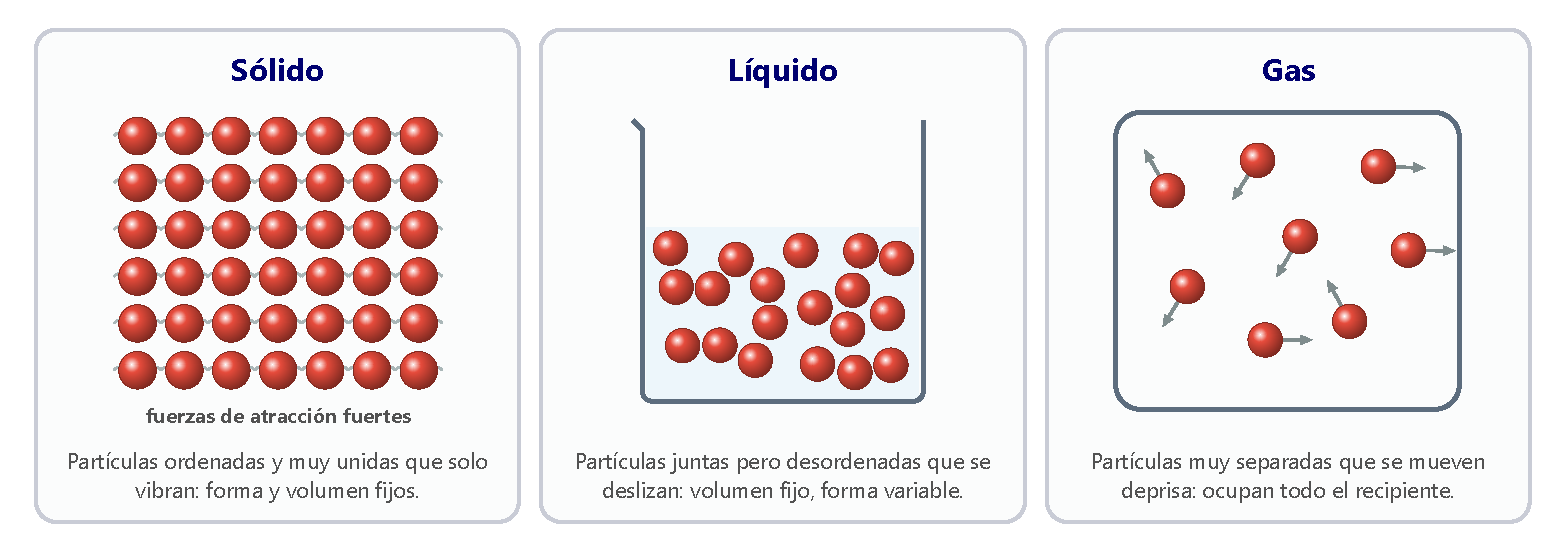
\includegraphics[width=0.85\textwidth]{images/UD1/estados_materia}
    \caption{Modelo de partículas de los tres estados de agregación.}
    \label{fig:ud1-estados}
\end{figure}

\paragraph{Temperatura, presión y volumen.} En el Sistema Internacional la temperatura se mide en \textbf{kelvin}:
\(T(\unit{\kelvin}) = t(\unit{\degreeCelsius}) + 273\). Una variación de \qty{1}{\degreeCelsius} equivale a una de
\qty{1}{\kelvin}. La \textbf{presión} es la fuerza perpendicular por unidad de superficie, \(p = F/S\); su unidad en el SI es el
\textbf{pascal} (\(\qty{1}{\pascal} = \qty{1}{\newton\per\square\metre}\)). La de un gas se debe a los choques de sus partículas
contra las paredes. Con su barómetro de mercurio, \textbf{Torricelli} demostró en 1643 que el aire pesa: al nivel del mar
sostiene una columna de mercurio de \qty{760}{\mm}. El \textbf{volumen} se mide en \unit{\cubic\metre}, aunque se usa mucho
el litro.

\begin{table}[H]
    \centering
    \caption{Equivalencias entre unidades de presión y de volumen}
    \vspace{-5pt}
    \begin{tabular}{@{}ll@{}}
        \toprule
        \textbf{Presión} & \textbf{Volumen} \\
        \midrule
        \(\qty{1}{\atm} = \qty{1.013e5}{\pascal}\) & \(\qty{1}{\cubic\metre} = \qty{1000}{\litre}\) \\[3pt]
        \(\qty{1}{\atm} = \qty{1.013}{\bar} = \qty{1013}{\milli\bar}\) & \(\qty{1}{\cubic\deci\metre} = \qty{1}{\litre}\) \\[3pt]
        \(\qty{1}{\atm} = \qty{760}{\mmHg}\) & \(\qty{1}{\cubic\centi\metre} = \qty{1}{\milli\litre}\) \\
        \bottomrule
    \end{tabular}
    \label{tab:ud1-unidades}
\end{table}

%========================================================================================
\section{Leyes ponderales}\label{sec:ud1-ponderales}
%========================================================================================

Las \textbf{leyes ponderales} son las leyes experimentales que relacionan las \textbf{masas} de las sustancias que intervienen
en una reacción química. Se descubrieron a finales del siglo \textsc{xviii} y comienzos del \textsc{xix}, cuando las balanzas
permitieron pesar con precisión.

\subsection{Ley de conservación de la masa o de Lavoisier}

\textbf{Antoine L. Lavoisier} (1743-1794) quería explicar por qué unas sustancias, como la madera, pierden masa al arder,
mientras que los metales, al calentarlos en el aire, se cubren de una capa de óxido y ganan masa. En su época se aceptaba la
teoría del \textbf{flogisto}: un fluido invisible que las sustancias ganaban o perdían al calentarse.

Lavoisier calentó estaño en un \textbf{recipiente cerrado} con aire. El estaño se transformó en un polvo (un óxido), pero la
masa del recipiente con todo su contenido \textbf{no cambió} (figura~\ref{fig:ud1-lavoisier}). Al abrirlo entraba aire, y la
masa del óxido era mayor que la del estaño inicial: el metal había tomado algo del aire, un componente que él mismo llamó
\textbf{oxígeno}. Este y otros experimentos le llevaron a enunciar:

\begin{definition}[Ley de conservación de la masa]
    En una reacción química, la masa total de las sustancias que intervienen permanece constante: la suma de las masas de los
    \textbf{reactivos} es igual a la suma de las masas de los \textbf{productos}.
\end{definition}

\begin{figure}[H]
    \centering
    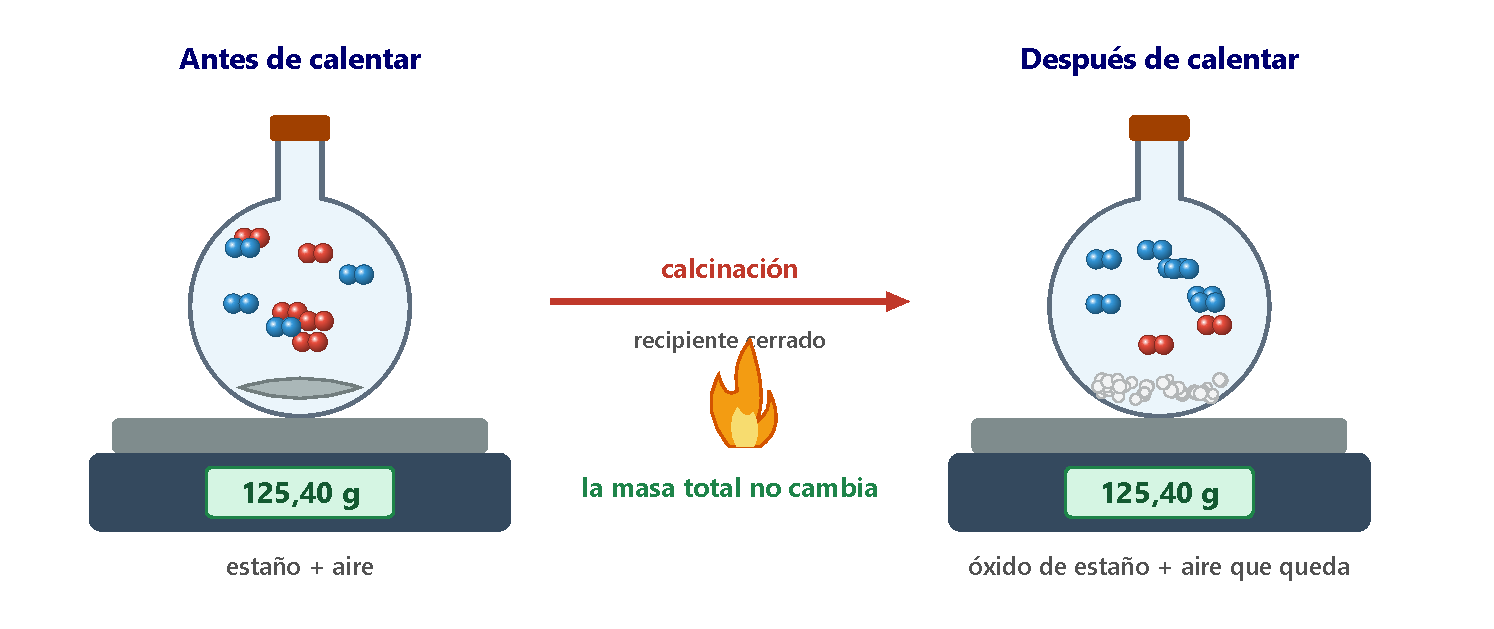
\includegraphics[width=0.85\textwidth]{images/UD1/conservacion_masa}
    \caption{El experimento de Lavoisier: al calcinar estaño en un recipiente cerrado, la masa total no cambia.}
    \label{fig:ud1-lavoisier}
\end{figure}

\begin{remark}
    La ley de Lavoisier no se cumple de forma exacta en las reacciones nucleares, en las que una pequeña parte de la masa se
    transforma en energía según la ecuación de Einstein, \(E = m c^2\). En las reacciones químicas esa variación es tan
    pequeña que no se puede medir.
\end{remark}

\begin{exercise}
    El carbono y el oxígeno se combinan para formar dióxido de carbono. Completa la tabla, sabiendo que en cada experiencia
    reaccionan completamente las masas indicadas.
    \begin{center}
        \begin{tabular}{@{}ccc@{}}
            \toprule
            \textbf{Carbono (g)} & \textbf{Oxígeno (g)} & \textbf{Dióxido de carbono (g)} \\
            \midrule
            12 & 32 & A \\[3pt]
            6 & B & 22 \\[3pt]
            C & 8 & 11 \\
            \bottomrule
        \end{tabular}
    \end{center}
    \begin{solu}
        \textcolor{blue}{Por la ley de Lavoisier, \(m_{\ch{C}} + m_{\ch{O}} = m_{\ch{CO2}}\):}
        \(A = 12 + 32 = \textcolor{red}{\qty{44}{\gram}}\); \(B = 22 - 6 = \textcolor{red}{\qty{16}{\gram}}\);
        \(C = 11 - 8 = \textcolor{red}{\qty{3}{\gram}}\).
    \end{solu}
\end{exercise}

\subsection{Ley de las proporciones definidas o de Proust}

El farmacéutico y químico francés \textbf{Joseph L. Proust} (1754-1826), que trabajó muchos años en España, analizó el
carbonato de cobre(II), \ch{CuCO3}, y comprobó que \textbf{cualquier muestra} contenía 5,3 partes de cobre, 1 de carbono y 4
de oxígeno, tanto si se había preparado en el laboratorio como si se había extraído de un mineral.

\begin{definition}[Ley de las proporciones definidas]
    Cuando dos o más elementos se combinan para formar un determinado compuesto, lo hacen siempre en una
    \textbf{proporción en masa fija}, independientemente del método de obtención o del estado físico del compuesto:
    \[ \frac{m_{\text{elemento A}}}{m_{\text{elemento B}}} = \text{constante} \]
\end{definition}

En el carbonato de cobre(II), la relación entre las masas de cobre y oxígeno es \(5{,}3/4 = \num{1.325}\). Esto permite
calcular la masa de un elemento conociendo la del otro: si una muestra contiene \qty{12}{\gram} de oxígeno, contiene
\(\num{1.325} \cdot 12 = \qty{15.9}{\gram}\) de cobre.

\begin{example}
    \textbf{Combinación del sodio y el cloro.} \qty{46}{\gram} de sodio reaccionan exactamente con \qty{71}{\gram} de cloro para
    dar cloruro de sodio. a) ¿En qué proporción en masa se combinan? b) ¿Cuántos gramos de cloro hacen falta para \qty{30}{\gram}
    de sodio?

    \textbf{Solución.} a) \(\dfrac{m_{\ch{Na}}}{m_{\ch{Cl}}} = \dfrac{46}{71} = \num{0.648}\): \num{0.648} g de sodio por cada
    gramo de cloro. También se puede dar al revés: \(\dfrac{m_{\ch{Cl}}}{m_{\ch{Na}}} = \dfrac{71}{46} = \num{1.54}\) g de cloro
    por cada gramo de sodio.

    b) La proporción se mantiene: \(\dfrac{m_{\ch{Cl}}}{30} = \dfrac{71}{46} \Rightarrow m_{\ch{Cl}} = \dfrac{71 \cdot 30}{46} =
    \qty{46.3}{\gram}\) de cloro.
\end{example}

\begin{exercise}
    \qty{42}{\gram} de hierro reaccionan con \qty{18}{\gram} de oxígeno para formar un óxido. ¿En qué proporción se combinan el
    hierro y el oxígeno?
    \begin{solu}
        \(\dfrac{m_{\ch{Fe}}}{m_{\ch{O}}} = \dfrac{42}{18} = \textcolor{red}{\dfrac{7}{3} = \num{2.33}}\): \textcolor{blue}{7 g de
        hierro por cada 3 g de oxígeno.}
    \end{solu}
\end{exercise}

\begin{exercise}
    El hierro y el azufre forman sulfuro de hierro(II) en una proporción en masa \(7:4\). ¿Cuántos gramos de hierro hacen
    falta para que reaccionen \qty{60}{\gram} de azufre?
    \begin{solu}
        \(\dfrac{m_{\ch{Fe}}}{m_{\ch{S}}} = \dfrac{7}{4} \Rightarrow m_{\ch{Fe}} = \dfrac{7 \cdot 60}{4} =
        \textcolor{red}{\qty{105}{\gram}}\) de hierro.
    \end{solu}
\end{exercise}

\subsection{Ley de las proporciones múltiples o de Dalton}

Algunos químicos de la época, como \textbf{Berthollet} (1748-1822), dudaron de la ley de Proust, porque observaban que dos
elementos podían unirse en \textbf{proporciones distintas} según las condiciones. Al quemar carbón en un lugar bien ventilado,
el gas que se forma tiene 8 partes de oxígeno por cada 3 de carbono; si hay poco oxígeno, tiene 4 partes de oxígeno por cada
3 de carbono.

\textbf{John Dalton} (1766-1844) dio con la explicación: no es un mismo compuesto con proporciones variables, sino \textbf{dos
compuestos diferentes}, el dióxido de carbono, \ch{CO2}, y el monóxido de carbono, \ch{CO}, y cada uno cumple la ley de
Proust. Además, observó que las masas de oxígeno que se combinan con la misma masa de carbono (3 g) guardan una relación muy
sencilla: \(8/4 = 2/1\).

\begin{definition}[Ley de las proporciones múltiples]
    Cuando dos elementos se combinan entre sí para formar más de un compuesto, las masas de un elemento que se combinan con
    una masa fija del otro guardan entre sí una relación de \textbf{números enteros sencillos}.
\end{definition}

\begin{example}
    \textbf{Agua y agua oxigenada.} En el agua, \qty{2}{\gram} de hidrógeno se combinan con \qty{16}{\gram} de oxígeno; en el
    agua oxigenada, \qty{3}{\gram} de hidrógeno se combinan con \qty{48}{\gram} de oxígeno. a) Comprueba que se cumple la ley de
    las proporciones múltiples. b) ¿Cuánto oxígeno se combina con \qty{30}{\gram} de hidrógeno en cada compuesto?

    \textbf{Solución.} a) Calculamos la masa de oxígeno que se combina con \qty{1}{\gram} de hidrógeno en cada compuesto:
    \[ \text{agua: } \frac{16}{2} = \qty{8}{\gram}; \qquad \text{agua oxigenada: } \frac{48}{3} = \qty{16}{\gram}; \qquad
    \frac{8}{16} = \frac{1}{2} \]
    La relación es de números enteros sencillos (1:2): por cada gramo de hidrógeno, el agua oxigenada tiene el doble de
    oxígeno que el agua.

    b) En el agua, \(30 \cdot 8 = \qty{240}{\gram}\) de oxígeno; en el agua oxigenada, el doble: \qty{480}{\gram}.
\end{example}

\begin{exercise}
    En el laboratorio se obtienen dos cloruros de cromo distintos. En el primero, \qty{7.8}{\gram} de cromo se combinan con
    \qty{10.65}{\gram} de cloro; en el segundo, \qty{10.4}{\gram} de cromo se combinan con \qty{21.30}{\gram} de cloro.
    Demuestra que se cumple la ley de las proporciones múltiples.
    \begin{solu}
        \textcolor{blue}{Masa de cloro por gramo de cromo:} primer compuesto \(10{,}65/7{,}8 = \num{1.365}\) g; segundo
        compuesto \(21{,}30/10{,}4 = \num{2.048}\) g.
        \textcolor{blue}{Relación:} \(\dfrac{\num{2.048}}{\num{1.365}} = \num{1.5} = \textcolor{red}{\dfrac{3}{2}}\), \textcolor{red}{números
        enteros sencillos: se cumple la ley de Dalton} (son \ch{CrCl2} y \ch{CrCl3}).
    \end{solu}
\end{exercise}

%========================================================================================
\section{Teoría atómica de Dalton}\label{sec:ud1-dalton}
%========================================================================================

En los siglos \textsc{v} y \textsc{iv} a.\,C. los filósofos griegos se preguntaban si la materia se puede dividir
indefinidamente. El \textbf{atomismo} de \textbf{Leucipo} y \textbf{Demócrito} sostenía que no: que todo está formado por
partículas diminutas e indivisibles, los \emph{átomos}. La \textbf{teoría continuista} de \textbf{Aristóteles}, en cambio,
defendía que la materia se puede dividir sin límite y que todo está formado por cuatro elementos (tierra, agua, aire y fuego).
Fue la idea aceptada durante unos 2000 años.

A comienzos del siglo \textsc{xix}, \textbf{Dalton} se dio cuenta de que las leyes ponderales no encajaban con una materia
continua: si la materia pudiera dividirse sin límite, ¿por qué los elementos se combinan siempre en proporciones fijas? Retomó
la idea de discontinuidad y, en 1808, publicó su \textbf{teoría atómica}:

\begin{definition}[Postulados de la teoría atómica de Dalton]
    \leavevmode % el título de la definición en su propia línea, la lista debajo
    \begin{enumerate}[label=\numberballblue]
        \item Los elementos están formados por partículas extraordinariamente pequeñas e indivisibles, los \textbf{átomos}.
        \item Todos los átomos de un mismo elemento son \textbf{idénticos} (misma masa, mismo tamaño y mismas propiedades); los
        de elementos distintos tienen masa y propiedades diferentes.
        \item Los compuestos se forman por la unión de átomos de elementos distintos en una \textbf{relación de números enteros
        sencillos}, formando «átomos compuestos» (hoy diríamos \textbf{moléculas}).
        \item En una reacción química, los átomos ni se crean ni se destruyen: solo se \textbf{recombinan}.
    \end{enumerate}
\end{definition}

\begin{figure}[H]
    \centering
    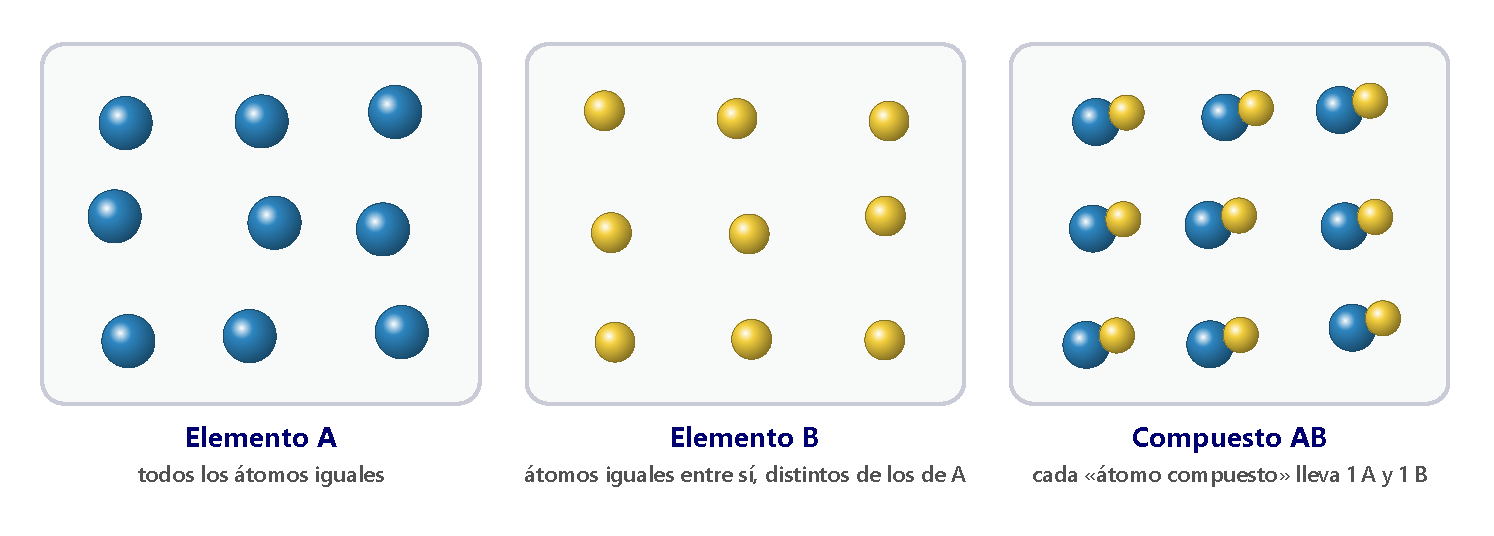
\includegraphics[width=0.85\textwidth]{images/UD1/dalton_teoria}
    \caption{Según Dalton, los átomos de un elemento son iguales entre sí, y un compuesto está formado por «átomos
    compuestos» idénticos.}
    \label{fig:ud1-dalton}
\end{figure}

\begin{remark}
    \textbf{¡Qué curioso!} Además de sus aportaciones a la química, Dalton fue el primero en describir la ceguera a los colores
    que él mismo padecía. Por eso, a esa alteración de la vista la llamamos \textbf{daltonismo}.
\end{remark}

\subsection{La teoría de Dalton explica las leyes ponderales}

\begin{itemize}
    \item \textbf{Conservación de la masa.} Por el postulado 4, en una reacción los átomos solo se recombinan. Antes y después
    hay los mismos átomos, así que la masa total no cambia. Por ejemplo, en \(\ch{2 S + C -> CS2}\), la masa del \ch{CS2} es la
    de dos átomos de azufre más la de uno de carbono.
    \item \textbf{Proporciones definidas.} Por el postulado 3, en un compuesto la relación entre el número de átomos de cada
    elemento es fija. En cualquier muestra de \ch{CO} hay un átomo de C por cada átomo de O, así que la relación entre las masas
    es siempre la de un átomo de C entre la de un átomo de O:
    \(\dfrac{m(\text{4 átomos de C})}{m(\text{4 átomos de O})} = \dfrac{m(\text{átomo de C})}{m(\text{átomo de O})}\).
    \item \textbf{Proporciones múltiples.} Como los átomos no se pueden dividir (postulado 1), una molécula contiene un número
    entero de átomos de cada elemento. En \ch{SO}, \ch{SO2} y \ch{SO3}, las masas de oxígeno unidas a un átomo de azufre son una,
    dos y tres veces la masa de un átomo de oxígeno: relación \(1:2:3\).
\end{itemize}

\begin{figure}[H]
    \centering
    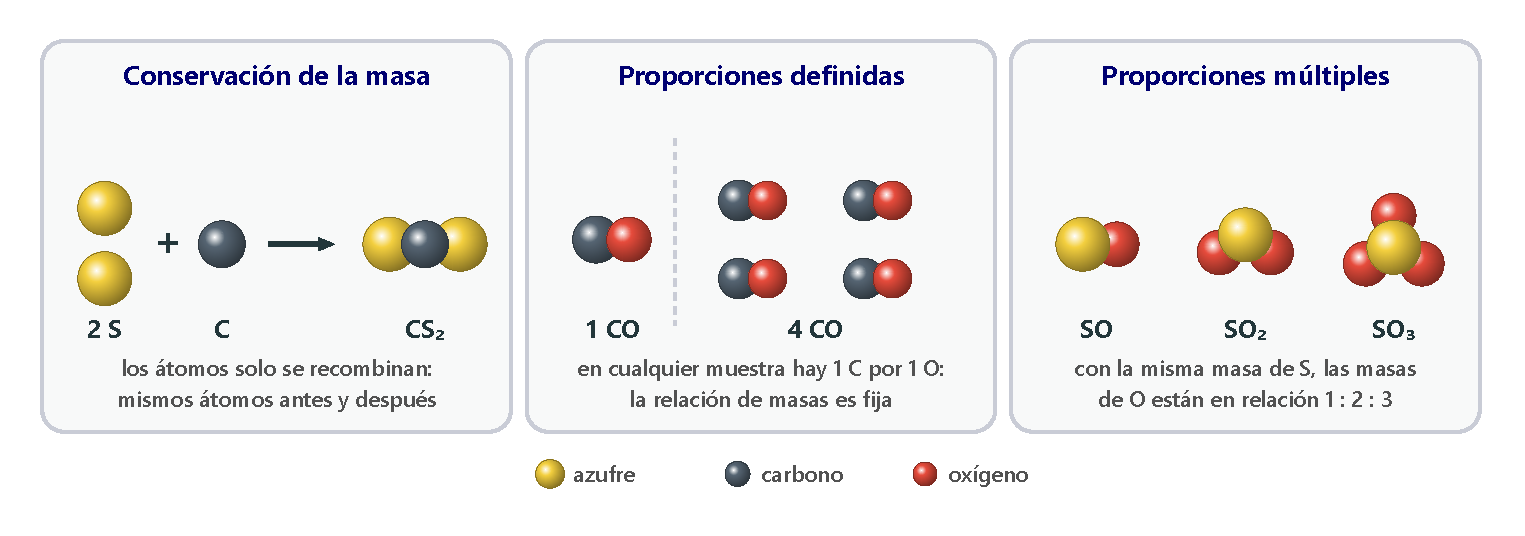
\includegraphics[width=0.9\textwidth]{images/UD1/dalton_leyes}
    \caption{Interpretación de las leyes ponderales con la teoría atómica de Dalton.}
    \label{fig:ud1-dalton-leyes}
\end{figure}

\subsection{Limitaciones de la teoría de Dalton}

La teoría atómica de Dalton fue un gran avance, pero hoy sabemos que tiene errores:
\begin{itemize}
    \item El átomo \textbf{no es indivisible}: está formado por partículas subatómicas (protones, neutrones y electrones).
    \item No todos los átomos de un elemento son idénticos: existen \textbf{isótopos}, átomos del mismo elemento con el mismo
    número de protones pero distinto número de neutrones, y por tanto con distinta masa (el hidrógeno tiene tres: protio,
    deuterio y tritio).
    \item Dalton pensaba que los «átomos compuestos» tenían la composición más sencilla posible. Por eso supuso que el agua
    era \ch{HO} y no \ch{H2O}, y obtuvo masas atómicas erróneas.
\end{itemize}

%========================================================================================
\section{Leyes volumétricas}\label{sec:ud1-volumetricas}
%========================================================================================

Las leyes ponderales se cumplen en cualquier reacción química. Cuando los reactivos y los productos son \textbf{gases}, se
cumplen además unas leyes que relacionan sus \textbf{volúmenes}: la ley de Gay-Lussac y la hipótesis de Avogadro.

\subsection{Ley de los volúmenes de combinación o de Gay-Lussac}

El químico francés \textbf{Joseph L. Gay-Lussac} (1778-1850) midió los volúmenes de gases que reaccionan y se forman,
siempre a la \textbf{misma presión y temperatura}. Encontró, por ejemplo, que 1 L de hidrógeno se combina con 1 L de cloro y
se forman 2 L de cloruro de hidrógeno; que 2 L de hidrógeno reaccionan con 1 L de oxígeno y dan 2 L de vapor de agua; y que
3 L de hidrógeno reaccionan con 1 L de nitrógeno para dar 2 L de amoníaco (figura~\ref{fig:ud1-volumenes}).

\begin{definition}[Ley de los volúmenes de combinación]
    En las reacciones químicas entre gases, los volúmenes de las sustancias que intervienen, medidos en las mismas
    condiciones de presión y temperatura, guardan entre sí una relación de \textbf{números enteros sencillos}.
\end{definition}

Fíjate en que los volúmenes \textbf{no se conservan}: \(3 + 1 \neq 2\). Lo que se conserva es la masa.

\begin{figure}[H]
    \centering
    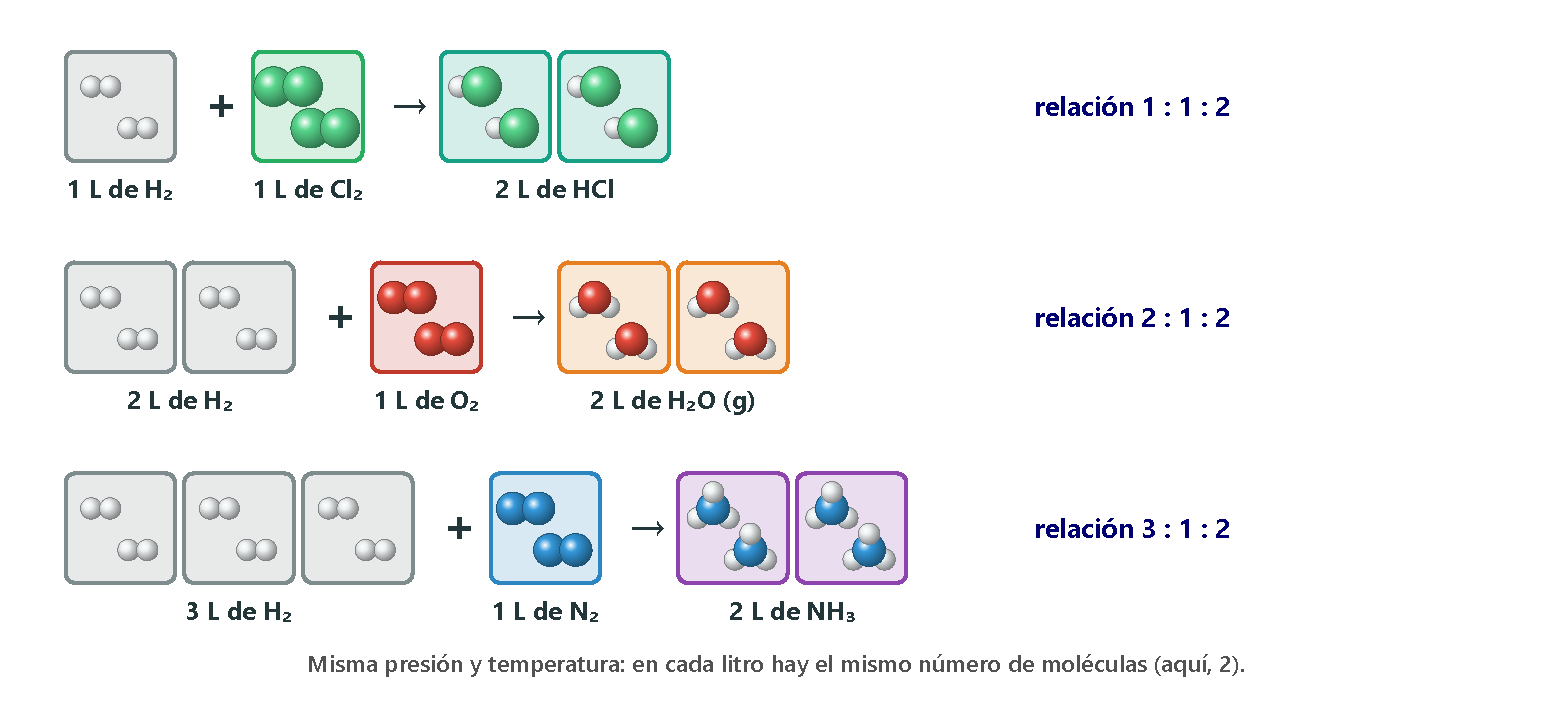
\includegraphics[width=0.9\textwidth]{images/UD1/volumenes_combinacion}
    \caption{Volúmenes de combinación de tres reacciones entre gases, interpretados con la hipótesis de Avogadro.}
    \label{fig:ud1-volumenes}
\end{figure}

\begin{example}
    \textbf{Combustión del monóxido de carbono.} \qty{6}{\litre} de \ch{CO} se combinan con \qty{3}{\litre} de \ch{O2} y se
    obtienen \qty{6}{\litre} de \ch{CO2}, todo medido en las mismas condiciones. a) ¿En qué relación volumétrica reaccionan el
    \ch{CO} y el \ch{O2}? b) ¿Cuántos litros de \ch{CO} hacen falta para \qty{250}{\litre} de oxígeno?

    \textbf{Solución.} a) \(\dfrac{V_{\ch{CO}}}{V_{\ch{O2}}} = \dfrac{6}{3} = 2\): relación \(2:1\).
    b) \(\dfrac{V_{\ch{CO}}}{250} = \dfrac{2}{1} \Rightarrow V_{\ch{CO}} = \qty{500}{\litre}\).
\end{example}

\begin{exercise}
    \(\ch{N2}(g)\) y \(\ch{H2}(g)\) reaccionan para dar amoníaco, \(\ch{NH3}(g)\), en la relación de volúmenes \(1:3:2\).
    Completa la tabla (todos los volúmenes se miden en las mismas condiciones).
    \begin{center}
        \begin{tabular}{@{}ccc@{}}
            \toprule
            \(V(\ch{N2})\) \textbf{(L)} & \(V(\ch{H2})\) \textbf{(L)} & \(V(\ch{NH3})\) \textbf{(L)} \\
            \midrule
            2 & A & B \\[3pt]
            C & 12 & D \\[3pt]
            E & F & 5 \\
            \bottomrule
        \end{tabular}
    \end{center}
    \begin{solu}
        \textcolor{blue}{Con la relación \(1:3:2\):} \(A = 3 \cdot 2 = \textcolor{red}{6}\); \(B = 2 \cdot 2 = \textcolor{red}{4}\);
        \(C = 12/3 = \textcolor{red}{4}\); \(D = 2 \cdot 4 = \textcolor{red}{8}\); \(E = 5/2 = \textcolor{red}{\num{2.5}}\);
        \(F = 3 \cdot \num{2.5} = \textcolor{red}{\num{7.5}}\) (en litros).
    \end{solu}
\end{exercise}

\subsection{La hipótesis de Avogadro}

El italiano \textbf{Amedeo Avogadro} (1776-1856), al estudiar los resultados de Gay-Lussac, pensó que el volumen de un gas
debía estar relacionado con el número de partículas que contiene.

\begin{definition}[Hipótesis de Avogadro]
    Volúmenes iguales de gases diferentes, medidos en las mismas condiciones de presión y temperatura, contienen el
    \textbf{mismo número de partículas}.
\end{definition}

Esta idea parecía chocar con la teoría de Dalton. Si el hidrógeno y el cloro fueran átomos sueltos, de 1 átomo de H y 1 de Cl
saldría 1 «átomo compuesto» de \ch{HCl}, y por tanto de 1 volumen de H y 1 de Cl saldría \textbf{un} volumen de \ch{HCl}. Pero
Gay-Lussac había medido \textbf{dos}. Avogadro resolvió el problema: las partículas de muchos gases no son átomos aislados,
sino agrupaciones de átomos, a las que llamó \textbf{moléculas}. Si el hidrógeno, el cloro, el oxígeno y el nitrógeno son
\textbf{diatómicos} (\ch{H2}, \ch{Cl2}, \ch{O2}, \ch{N2}), todo encaja:
\[ \ch{H2 + Cl2 -> 2 HCl} \qquad \ch{2 H2 + O2 -> 2 H2O} \qquad \ch{3 H2 + N2 -> 2 NH3} \]
Una molécula de \ch{H2} y una de \ch{Cl2} se rompen y se recombinan en dos moléculas de \ch{HCl}; y la misma relación (1:1:2)
aparece entre los volúmenes. Confirmada experimentalmente, la hipótesis de Avogadro pasó a ser una \textbf{ley}.

\begin{example}
    \textbf{Síntesis del amoníaco.} \qty{2}{\litre} de nitrógeno reaccionan con \qty{6}{\litre} de hidrógeno y se obtienen
    \qty{4}{\litre} de amoníaco. Justifica que se cumple la hipótesis de Avogadro.

    \textbf{Solución.} La relación de volúmenes es \(2:6:4 = 1:3:2\). Si en cada litro hay el mismo número de moléculas, por
    cada molécula de \ch{N2} reaccionan 3 de \ch{H2} y se forman 2 de \ch{NH3}: \(\ch{N2 + 3 H2 -> 2 NH3}\). Los átomos cuadran
    (2 de N y 6 de H a cada lado) si cada molécula de amoníaco tiene un átomo de nitrógeno y tres de hidrógeno, que es lo que
    se observa. Por tanto, los datos son coherentes con la hipótesis de Avogadro.
\end{example}

\begin{exercise}
    Al reaccionar \qty{8}{\litre} de hidrógeno con \qty{4}{\litre} de oxígeno se obtienen \qty{8}{\litre} de vapor de agua,
    medidos en las mismas condiciones. Justifica con la hipótesis de Avogadro que la fórmula del agua es \ch{H2O}.
    \begin{solu}
        \textcolor{blue}{Relación de volúmenes \(8:4:8 = 2:1:2\). Si cada litro contiene el mismo número de moléculas, 2 moléculas
        de \ch{H2} y 1 de \ch{O2} dan 2 moléculas de agua: \(\ch{2 H2 + O2 -> 2 H2O}\).} Para que los átomos cuadren (4 de H y 2 de O),
        \textcolor{red}{cada molécula de agua debe tener 2 átomos de H y 1 de O: \ch{H2O}}.
    \end{solu}
\end{exercise}

%========================================================================================
\section{La cantidad de sustancia}\label{sec:ud1-mol}
%========================================================================================

Los átomos son tan pequeños que ninguna balanza puede pesar uno solo. ¿Cómo podemos entonces asignarles una masa? Recuerda
que \textbf{medir es comparar} con una cantidad que tomamos como patrón.

\subsection{Masas atómicas y moleculares}

En el siglo \textsc{xix}, Dalton y otros químicos determinaron la masa de los átomos \textbf{comparándolos entre sí}. Así
averiguaron que el hidrógeno era el más ligero y construyeron una tabla con la masa de cada elemento referida a la del
hidrógeno. Hoy, por acuerdo internacional, el patrón es el átomo de carbono-12 (\(^{12}\)C), al que se asigna una masa de 12
unidades (figura~\ref{fig:ud1-masa-atomica}).

\begin{definition}[Masa atómica relativa]
    La \textbf{masa atómica relativa} de un elemento, \(A_r\), es el número de veces que la masa de uno de sus átomos contiene
    a la doceava parte de la masa de un átomo de \(^{12}\)C:
    \[ A_r = \frac{\text{masa de un átomo del elemento}}{\frac{1}{12}\,(\text{masa de un átomo de } ^{12}\text{C})} \]
\end{definition}

\(A_r\) es un número \textbf{sin unidades}, porque es el cociente de dos masas. En 1960 la IUPAC definió la
\textbf{unidad de masa atómica}, \unit{\uma}, como la doceava parte de la masa de un átomo de \(^{12}\)C:
\[ \qty{1}{\uma} = \qty{1.6605e-27}{\kilogram} \]
La \textbf{masa atómica} de un elemento, \(A\), es la masa de uno de sus átomos expresada en \unit{\uma}. Tiene unidades, pero
coincide numéricamente con \(A_r\): \(A_r(\ch{O}) = 16\) y \(A(\ch{O}) = \qty{16}{\uma}\).

\begin{figure}[H]
    \centering
    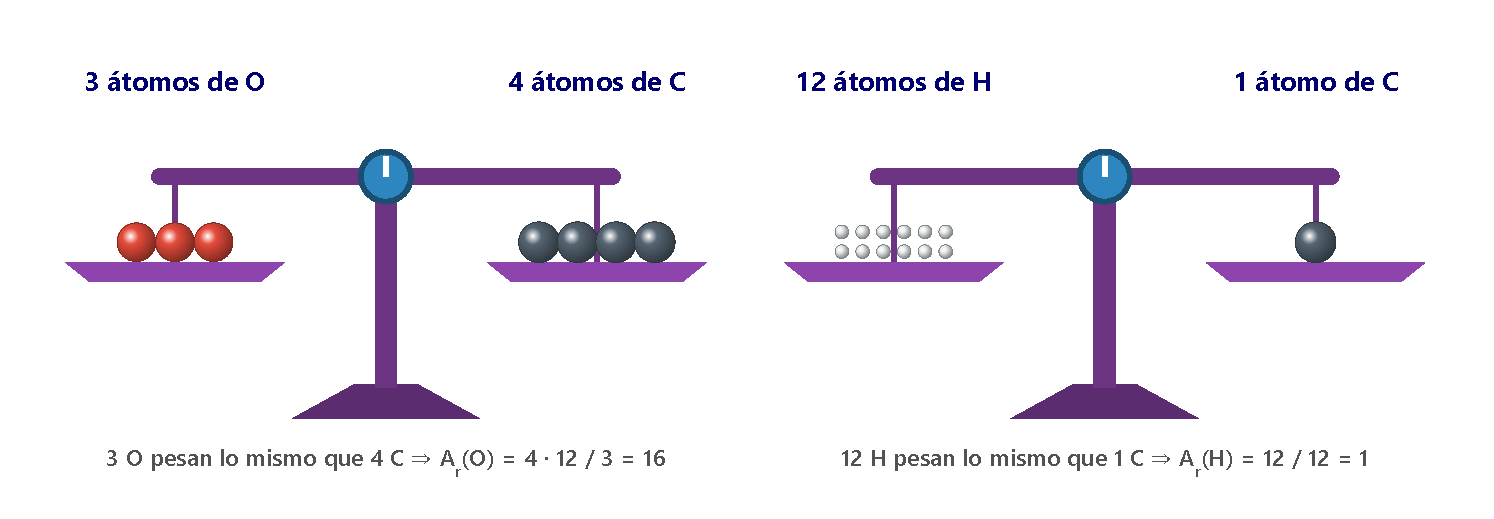
\includegraphics[width=0.85\textwidth]{images/UD1/masa_atomica}
    \caption{Si 3 átomos de oxígeno tienen la misma masa que 4 de carbono (12 cada uno), cada átomo de oxígeno tiene una masa
    relativa de 16.}
    \label{fig:ud1-masa-atomica}
\end{figure}

La \textbf{fórmula} de una sustancia indica los elementos que la forman y la proporción de átomos de cada uno. La masa de una
molécula es la suma de las masas de sus átomos:

\begin{definition}[Masa molecular relativa]
    La \textbf{masa molecular relativa} de un compuesto, \(M_r\), es la suma de las masas atómicas relativas de los átomos que
    forman su molécula. En los compuestos que no forman moléculas (los iónicos, como el \ch{NaCl}, o los cristales covalentes)
    se habla de \textbf{masa fórmula relativa}, calculada con la unidad fórmula.
\end{definition}

Por ejemplo, \(M_r(\ch{H2O}) = 2 \cdot A_r(\ch{H}) + A_r(\ch{O}) = 2 \cdot 1 + 16 = 18\) y
\(M_r(\ch{CO2}) = 12 + 2 \cdot 16 = 44\).

\begin{example}
    \textbf{Masas moleculares.} Calcula la masa molecular de: a) ácido sulfúrico, \ch{H2SO4}; b) etano, \ch{C2H6}; c) nitrógeno,
    \ch{N2}.

    \textbf{Solución.} a) \(M(\ch{H2SO4}) = 2 \cdot 1 + 32 + 4 \cdot 16 = \qty{98}{\uma}\);
    b) \(M(\ch{C2H6}) = 2 \cdot 12 + 6 \cdot 1 = \qty{30}{\uma}\);
    c) \(M(\ch{N2}) = 2 \cdot 14 = \qty{28}{\uma}\).
\end{example}

\subsection{El mol}

Una \textbf{docena} son 12 unidades, sean lápices o huevos. Una docena de lápices y una docena de gomas tienen el mismo número
de objetos, pero distinta masa. Con el \textbf{mol} ocurre lo mismo, pero el número de objetos es enorme, porque los átomos son
diminutos: para tener una cantidad que se pueda pesar con una balanza hacen falta muchísimos.

\begin{definition}[Mol]
    El \textbf{mol} es la unidad de \textbf{cantidad de sustancia} en el Sistema Internacional. Un mol contiene exactamente
    \num{6.022e23} entidades elementales (átomos, moléculas, iones, electrones…). Ese número es el valor de la
    \textbf{constante de Avogadro}:
    \[ N_A = \qty{6.022e23}{\per\mole} \]
\end{definition}

Inicialmente el mol se definió como el número de átomos que hay en \qty{12}{\gram} de \(^{12}\)C; ese número se midió por
varios métodos y resultó ser \num{6.022e23}. Un mol de átomos de carbono contiene \num{6.022e23} átomos de C. Un mol de
moléculas de metano, \ch{CH4}, contiene \num{6.022e23} moléculas, que suman \num{6.022e23} átomos de C y
\(4 \cdot \num{6.022e23} = \num{2.409e24}\) átomos de H.

\begin{remark}
    Un mol de \ch{HCl} y un mol de \ch{H2O} tienen el mismo número de moléculas, pero distinta masa (\qty{36.5}{\gram} y
    \qty{18}{\gram}), igual que una docena de lápices y una docena de gomas.
\end{remark}

\subsection{La masa molar}

\begin{definition}[Masa molar]
    La \textbf{masa molar}, \(M\), de una sustancia es la masa de un mol de sus partículas. Se suele expresar en
    \unit{\gram\per\mole} (en el SI, \unit{\kilogram\per\mole}).
\end{definition}

Como un mol de \(^{12}\)C tiene una masa de \qty{12}{\gram} y cada átomo «vale» 12 unidades, la masa molar de cualquier
sustancia, en \unit{\gram\per\mole}, es \textbf{numéricamente igual} a su masa atómica o molecular relativa. Para el metano:
\(M_r(\ch{CH4}) = 12 + 4 \cdot 1 = 16\), luego \(M(\ch{CH4}) = \qty{16}{\gram\per\mole}\).

\subsection{Cálculos con moles}

La cantidad de sustancia, \(n\), la masa, \(m\), y el número de partículas, \(N\), son directamente proporcionales. Conocida
una de ellas, se calculan las otras con estas fórmulas o con factores de conversión (figura~\ref{fig:ud1-mol}):
\[ n = \frac{m}{M} \qquad\qquad n = \frac{N}{N_A} \]

\begin{figure}[H]
    \centering
    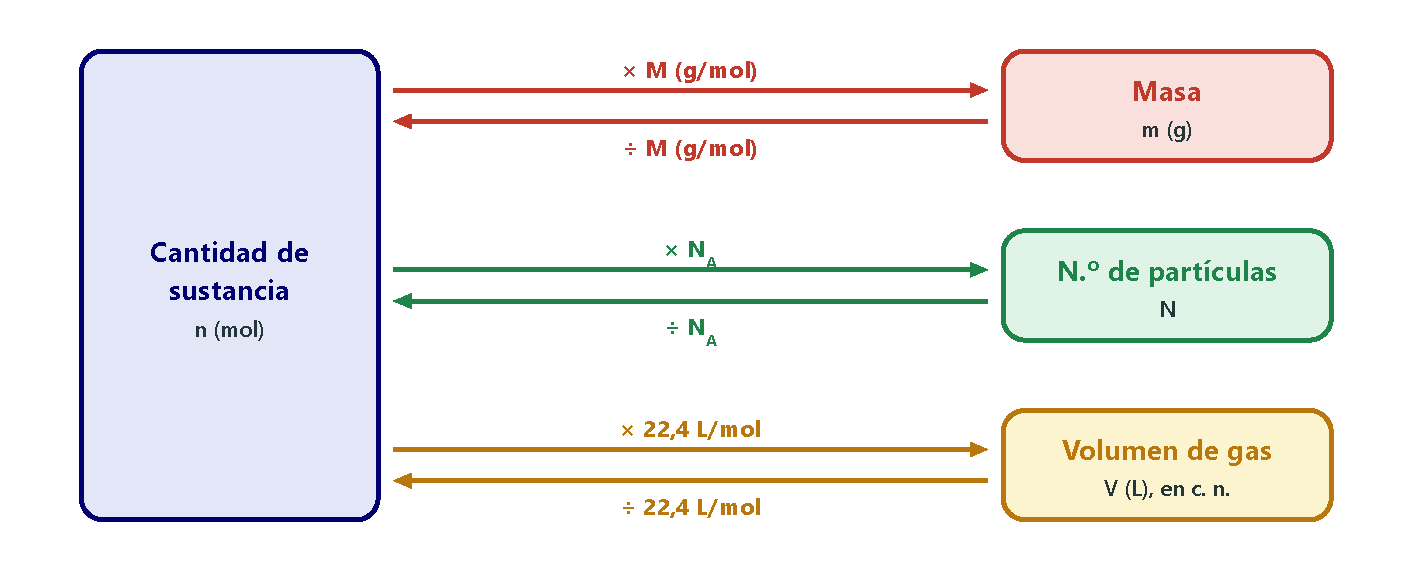
\includegraphics[width=0.75\textwidth]{images/UD1/mol_gas}
    \caption{El mol relaciona la masa, el número de partículas y, en los gases, el volumen (apartado~\ref{sec:ud1-gases-ideales}).}
    \label{fig:ud1-mol}
\end{figure}

\begin{example}
    \textbf{Azúcar en un refresco.} Una lata de refresco lleva el equivalente a 7 terrones de azúcar de \qty{4}{\gram} de
    glucosa, \ch{C6H12O6}, cada uno. Calcula: a) la masa molar de la glucosa; b) los moles de glucosa de la lata; c) los átomos de
    carbono; d) los moles de átomos de oxígeno; e) la masa de hidrógeno; f) la masa de 5 moles de glucosa; g) la masa de glucosa
    que contiene \num{2.4e25} átomos de oxígeno; h) la masa de glucosa que contiene \qty{90}{\gram} de carbono.

    \textbf{Solución.} a) \(M(\ch{C6H12O6}) = 6 \cdot 12 + 12 \cdot 1 + 6 \cdot 16 = \qty{180}{\gram\per\mole}\).

    b) La lata tiene \(7 \cdot 4 = \qty{28}{\gram}\) de glucosa:
    \(\qty{28}{\gram} \cdot \dfrac{\qty{1}{\mole}}{\qty{180}{\gram}} = \qty{0.156}{\mole}\).

    c) \(\qty{0.156}{\mole} \cdot \dfrac{\text{6 mol C}}{\text{1 mol glucosa}} \cdot \dfrac{\num{6.022e23}\text{ átomos}}{\text{1 mol}}
    = \num{5.62e23}\) átomos de C.

    d) \(\qty{0.156}{\mole} \cdot \dfrac{\text{6 mol O}}{\text{1 mol glucosa}} = \qty{0.933}{\mole}\) de átomos de O.

    e) En \qty{180}{\gram} de glucosa hay \qty{12}{\gram} de H: \(28 \cdot \dfrac{12}{180} = \qty{1.87}{\gram}\) de H.

    f) \(\qty{5}{\mole} \cdot \qty{180}{\gram\per\mole} = \qty{900}{\gram}\).

    g) \(\num{2.4e25}\text{ átomos O} \cdot \dfrac{\text{1 mol O}}{\num{6.022e23}\text{ átomos}} \cdot
    \dfrac{\text{1 mol glucosa}}{\text{6 mol O}} \cdot \dfrac{\qty{180}{\gram}}{\text{1 mol glucosa}} = \qty{1196}{\gram}\).

    h) Cada \qty{180}{\gram} de glucosa contienen \(6 \cdot 12 = \qty{72}{\gram}\) de C:
    \(\qty{90}{\gram}\text{ C} \cdot \dfrac{\qty{180}{\gram}\text{ glucosa}}{\qty{72}{\gram}\text{ C}} = \qty{225}{\gram}\) de glucosa.
\end{example}

\begin{exercise}
    En una muestra de \qty{20}{\gram} de sodio, ¿cuántos moles y cuántos átomos de sodio hay?
    \begin{solu}
        \(n = \dfrac{20}{23} = \textcolor{red}{\qty{0.870}{\mole}}\);
        \(N = \num{0.870} \cdot \num{6.022e23} = \textcolor{red}{\num{5.24e23}}\) \textcolor{red}{átomos de Na}.
    \end{solu}
\end{exercise}

\begin{exercise}
    Una olla a presión contiene \num{9.5e23} partículas de aire (78\,\% de \ch{N2} y 21\,\% de \ch{O2}, en número de
    partículas). ¿Cuántas moléculas de cada gas hay?
    \begin{solu}
        \(N(\ch{N2}) = \num{0.78} \cdot \num{9.5e23} = \textcolor{red}{\num{7.41e23}}\);
        \(N(\ch{O2}) = \num{0.21} \cdot \num{9.5e23} = \textcolor{red}{\num{2.00e23}}\) moléculas.
    \end{solu}
\end{exercise}

\begin{exercise}
    Una joya de un metal precioso contiene \num{3.5e23} átomos y tiene una masa de \qty{62.7}{\gram}. a) Calcula la masa molar
    del metal. b) ¿De qué metal se trata?
    \begin{solu}
        a) \(n = \dfrac{\num{3.5e23}}{\num{6.022e23}} = \qty{0.581}{\mole}\);
        \(M = \dfrac{\qty{62.7}{\gram}}{\qty{0.581}{\mole}} = \textcolor{red}{\qty{107.9}{\gram\per\mole}}\).
        b) \textcolor{red}{Plata (Ag)}.
    \end{solu}
\end{exercise}

\begin{exercise}
    El análisis del agua de una laguna indica que hay \num{5e17} átomos de plomo por cada litro. Calcula: a) los átomos de Pb que
    hay en \qty{1}{\cubic\metre} de agua; b) la masa de plomo en \qty{1}{\cubic\metre} de agua.
    \begin{solu}
        a) \(\num{5e17} \cdot 1000 = \textcolor{red}{\num{5e20}}\) átomos.
        b) \(\dfrac{\num{5e20}}{\num{6.022e23}} \cdot \num{207.2} = \textcolor{red}{\qty{0.172}{\gram}}\) de Pb.
    \end{solu}
\end{exercise}

\begin{exercise}
    Una botella de agua contiene \num{4.8e25} átomos de hidrógeno. ¿Qué masa de agua contiene?
    \begin{solu}
        \textcolor{blue}{Cada molécula de \ch{H2O} tiene 2 átomos de H:} \(N(\ch{H2O}) = \num{2.4e25}\) moléculas;
        \(n = \dfrac{\num{2.4e25}}{\num{6.022e23}} = \qty{39.85}{\mole}\); \(m = \num{39.85} \cdot 18 = \qty{717}{\gram} =
        \textcolor{red}{\qty{0.717}{\kilogram}}\).
    \end{solu}
\end{exercise}

%========================================================================================
\section{La fórmula de las sustancias}\label{sec:ud1-formula}
%========================================================================================

La \textbf{fórmula química} indica los elementos que forman una sustancia y la proporción en que están. Hay dos tipos:

\begin{table}[H]
    \centering
    \caption{Fórmula empírica y fórmula molecular}
    \vspace{-5pt}
    \begin{tabular}{@{}L{7cm}L{7cm}@{}}
        \toprule
        \textbf{Fórmula empírica} & \textbf{Fórmula molecular} \\
        \midrule
        Indica qué elementos forman la sustancia y la \textbf{proporción más sencilla}, en números enteros, en que se combinan
        sus átomos. &
        Indica el \textbf{número exacto} de átomos de cada elemento que hay en una molécula. Es un múltiplo entero de la
        empírica. \\[3pt]
        Ácido acético: \ch{CH2O} (por cada átomo de C hay 2 de H y 1 de O). &
        Ácido acético: \ch{C2H4O2} (cada molécula tiene 2 átomos de C, 4 de H y 2 de O). \\
        \bottomrule
    \end{tabular}
    \label{tab:ud1-formulas}
\end{table}

Todos los compuestos tienen fórmula empírica, pero solo los formados por \textbf{moléculas} tienen fórmula molecular. En un
compuesto iónico como el \ch{NaCl} la fórmula solo indica la proporción de iones en el cristal.

\subsection{Composición centesimal}

El hierro se extrae de minerales como la \textbf{hematita}, \ch{Fe2O3}, o la \textbf{siderita}, \ch{FeCO3}. ¿Cuál es más
rentable? El que tenga mayor porcentaje de hierro:
\begin{itemize}
    \item Hematita: \(M(\ch{Fe2O3}) = 2 \cdot \num{55.8} + 3 \cdot 16 = \qty{159.6}{\gram\per\mole}\); en \qty{159.6}{\gram} hay
    \(2 \cdot \num{55.8} = \qty{111.6}{\gram}\) de Fe: \(\%\,\ch{Fe} = \dfrac{\num{111.6}}{\num{159.6}} \cdot 100 = \qty{69.92}{\percent}\).
    \item Siderita: \(M(\ch{FeCO3}) = \num{55.8} + 12 + 3 \cdot 16 = \qty{115.8}{\gram\per\mole}\):
    \(\%\,\ch{Fe} = \dfrac{\num{55.8}}{\num{115.8}} \cdot 100 = \qty{48.19}{\percent}\).
\end{itemize}
La hematita tiene mayor \textbf{riqueza} en hierro.

\begin{definition}[Composición centesimal]
    La \textbf{composición centesimal} de un compuesto es el tanto por ciento en masa de cada elemento, es decir, los gramos de
    cada elemento que hay en \qty{100}{\gram} de compuesto:
    \[ \%\,(\text{elemento}) = \frac{\text{masa del elemento}}{\text{masa del compuesto}} \cdot 100 \]
\end{definition}

Por la ley de Proust, la composición centesimal de un compuesto es \textbf{fija}. Se puede calcular a partir de la masa molar
(como en los ejemplos anteriores) o a partir de cualquier muestra de la que conozcamos la masa total y la de cada elemento.

\subsection{Cálculo de la fórmula empírica}

La fórmula empírica indica la proporción en que se combinan los átomos, y esa misma proporción se da entre los
\textbf{moles} de átomos: en el \ch{Fe2O3}, 3 átomos de O se combinan con 2 de Fe, y 3 moles de O con 2 moles de Fe. Para
obtenerla a partir de la composición centesimal (o de las masas de una muestra):

\begin{enumerate}[label=\numberballblue]
    \item Divide la masa de cada elemento entre su masa atómica: obtienes los \textbf{moles de átomos} de cada uno.
    \item Divide todos los resultados entre el \textbf{más pequeño}: obtienes la relación entre ellos.
    \item Si algún número es decimal (por ejemplo 1,5 o 1,33), \textbf{multiplica} todos por el mismo entero (2, 3…) hasta que
    sean enteros. Esos son los subíndices.
    \item Escribe el símbolo de cada elemento con su subíndice.
\end{enumerate}

\subsection{Cálculo de la fórmula molecular}

La fórmula molecular es un múltiplo de la empírica: fórmula molecular \(= \alpha \cdot{}\)(fórmula empírica).
Para hallar el factor \(\alpha\) hace falta conocer la \textbf{masa molar real} del compuesto (en el apartado~\ref{sec:ud1-gases-ideales}
veremos cómo medirla en los gases):
\[ \alpha = \frac{\text{masa molar real}}{\text{masa molar de la fórmula empírica}} \]
Si la fórmula empírica es \ch{A2B3} y \(\alpha = 2\), la molecular es \ch{A4B6}.

\begin{example}
    \textbf{Fórmula de una sal.} Un compuesto contiene un 17,04\,\% de Na, un 47,41\,\% de S y un 35,55\,\% de O. Su masa molar es
    \qty{270}{\gram\per\mole}. Calcula: a) su fórmula empírica; b) su fórmula molecular.

    \textbf{Solución.} a) Tomamos \qty{100}{\gram} de compuesto y calculamos los moles de átomos de cada elemento; después
    dividimos entre el menor:
    \[ \ch{Na}: \frac{\num{17.04}}{23} = \num{0.741} \rightarrow 1; \qquad
       \ch{S}: \frac{\num{47.41}}{32} = \num{1.482} \rightarrow \frac{\num{1.482}}{\num{0.741}} = 2; \qquad
       \ch{O}: \frac{\num{35.55}}{16} = \num{2.222} \rightarrow \frac{\num{2.222}}{\num{0.741}} = 3 \]
    La fórmula empírica es \ch{NaS2O3}.

    b) \(M(\ch{NaS2O3}) = 23 + 2 \cdot 32 + 3 \cdot 16 = \qty{135}{\gram\per\mole}\); \(\alpha = 270/135 = 2\). La fórmula
    molecular es \ch{Na2S4O6} (tetrationato de sodio).
\end{example}

\begin{exercise}
    Una sal contiene un 40,21\,\% de potasio, un 26,80\,\% de cromo y un 32,99\,\% de oxígeno. Calcula su fórmula empírica.
    \begin{solu}
        \textcolor{blue}{Moles de átomos en \qty{100}{\gram}:} K \(\num{40.21}/39 = \num{1.031}\); Cr \(\num{26.80}/52 = \num{0.515}\);
        O \(\num{32.99}/16 = \num{2.062}\). \textcolor{blue}{Dividiendo entre \num{0.515}:} 2 : 1 : 4.
        \textcolor{red}{Fórmula empírica: \ch{K2CrO4}}.
    \end{solu}
\end{exercise}

\begin{exercise}
    Un compuesto orgánico contiene un 40,0\,\% de C, un 6,7\,\% de H y el resto de oxígeno. a) Calcula su fórmula empírica.
    b) Si \(\alpha = 6\), ¿cuál es su masa molar y su fórmula molecular?
    \begin{solu}
        a) \textcolor{blue}{O: \(100 - 40{,}0 - 6{,}7 = \qty{53.3}{\percent}\).} C \(40{,}0/12 = \num{3.33}\); H \(6{,}7/1 = \num{6.7}\);
        O \(53{,}3/16 = \num{3.33}\) \(\rightarrow\) 1 : 2 : 1. \textcolor{red}{Fórmula empírica: \ch{CH2O}}.
        b) \(M = 6 \cdot 30 = \textcolor{red}{\qty{180}{\gram\per\mole}}\); \textcolor{red}{fórmula molecular \ch{C6H12O6}}.
    \end{solu}
\end{exercise}

%========================================================================================
\section{Las leyes de los gases}\label{sec:ud1-leyes-gases}
%========================================================================================

Las bombonas de oxígeno, los airbags o las ollas a presión son dispositivos diseñados a partir del conocimiento del
comportamiento de los gases. El estado de una cantidad fija de gas queda determinado por tres magnitudes: su
\textbf{presión}, \(p\), su \textbf{volumen}, \(V\), y su \textbf{temperatura}, \(T\). Desde el siglo \textsc{xvii} varios
científicos estudiaron cómo se relacionan, manteniendo \textbf{fija una de ellas} y variando las otras dos
(figura~\ref{fig:ud1-leyes-gases}).

\begin{definition}[Leyes de los gases (para una cantidad fija de gas)]
    \leavevmode % el título de la definición en su propia línea, la lista debajo
    \begin{itemize}
        \item \textbf{Ley de Boyle-Mariotte.} A \textbf{temperatura constante}, el volumen de un gas es inversamente proporcional
        a la presión: \(\;p_1 V_1 = p_2 V_2 = \text{constante}\).
        \item \textbf{Ley de Gay-Lussac.} A \textbf{volumen constante}, la presión de un gas es directamente proporcional a su
        temperatura absoluta: \(\;\dfrac{p_1}{T_1} = \dfrac{p_2}{T_2} = \text{constante}\).
        \item \textbf{Ley de Charles.} A \textbf{presión constante}, el volumen de un gas es directamente proporcional a su
        temperatura absoluta: \(\;\dfrac{V_1}{T_1} = \dfrac{V_2}{T_2} = \text{constante}\).
    \end{itemize}
\end{definition}

\begin{figure}[H]
    \centering
    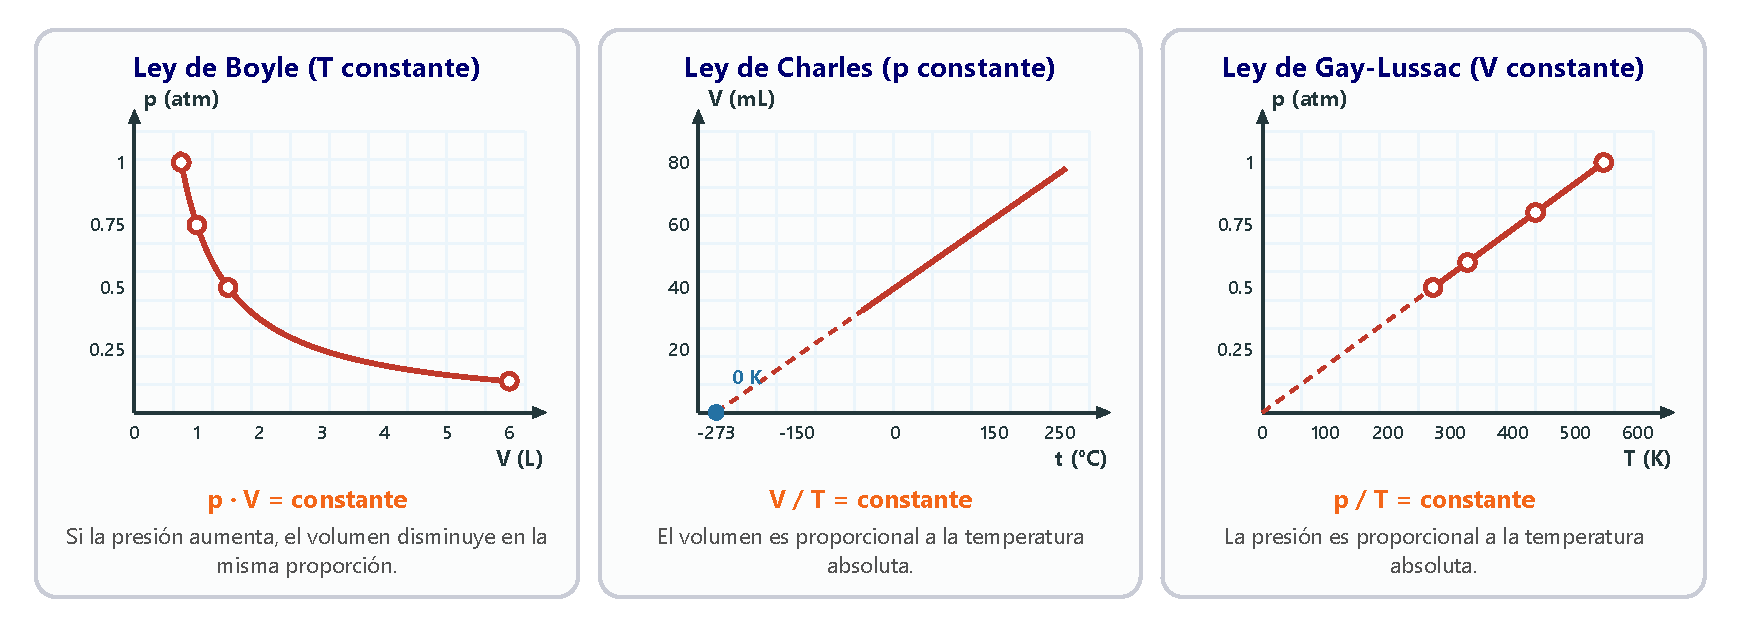
\includegraphics[width=\textwidth]{images/UD1/leyes_gases}
    \caption{Representación gráfica de las tres leyes de los gases.}
    \label{fig:ud1-leyes-gases}
\end{figure}

\begin{remark}
    \textbf{Ten en cuenta.} En las leyes de los gases la presión y el volumen pueden expresarse en cualquier unidad, siempre que
    sea la \textbf{misma} a ambos lados de la igualdad. La temperatura, en cambio, ha de estar siempre en \textbf{kelvin}.
\end{remark}

Si prolongamos hacia la izquierda la recta \(V\)-\(t\) de la ley de Charles, corta al eje de temperaturas en
\qty{-273}{\degreeCelsius}: es el \textbf{cero absoluto}, la temperatura más baja posible, origen de la escala Kelvin.

\begin{exercise}
    Un globo a \qty{850}{\mmHg} ocupa \qty{4}{\cubic\metre}. ¿Qué presión tendrá si reducimos su volumen a la mitad sin cambiar la
    temperatura?
    \begin{solu}
        \textcolor{blue}{Boyle: \(p_2 = p_1 V_1 / V_2 = 850 \cdot 4 / 2\)} \(= \qty{1700}{\mmHg} = \textcolor{red}{\qty{2.24}{\atm}}\).
    \end{solu}
\end{exercise}

\begin{exercise}
    En un recipiente de \qty{20}{\litre} la presión es de \qty{1500}{\milli\bar}. ¿Cuál será su volumen si la presión, a
    temperatura constante, aumenta hasta \qty{3e5}{\pascal}?
    \begin{solu}
        \textcolor{blue}{\(\qty{1500}{\milli\bar} = \qty{1.5e5}{\pascal}\).} \(V_2 = \dfrac{\num{1.5e5} \cdot 20}{\num{3e5}} =
        \textcolor{red}{\qty{10}{\litre}}\).
    \end{solu}
\end{exercise}

\begin{exercise}
    Un gas a \qty{25}{\degreeCelsius} y \qty{500}{\mmHg} se calienta a volumen constante hasta que su presión es de
    \qty{900}{\mmHg}. ¿Cuál es la temperatura final en \unit{\degreeCelsius}?
    \begin{solu}
        \textcolor{blue}{Gay-Lussac:} \(T_2 = T_1 \dfrac{p_2}{p_1} = 298 \cdot \dfrac{900}{500} = \qty{536.4}{\kelvin} =
        \textcolor{red}{\qty{263.4}{\degreeCelsius}}\).
    \end{solu}
\end{exercise}

\begin{exercise}
    La presión del aire en un matraz cerrado es de \qty{480}{\mmHg} a \qty{40}{\degreeCelsius}. ¿Cuál será la presión si se
    calienta hasta \qty{120}{\degreeCelsius}? Supón el volumen constante.
    \begin{solu}
        \(p_2 = p_1 \dfrac{T_2}{T_1} = 480 \cdot \dfrac{393}{313} = \qty{602.7}{\mmHg} = \textcolor{red}{\qty{0.793}{\atm}}\).
    \end{solu}
\end{exercise}

\begin{exercise}
    Un globo ocupa \qty{200}{\cubic\centi\metre} a \qty{10}{\degreeCelsius}. ¿Qué volumen ocuparía a \qty{35}{\degreeCelsius}, a la
    misma presión?
    \begin{solu}
        \textcolor{blue}{Charles:} \(V_2 = V_1 \dfrac{T_2}{T_1} = 200 \cdot \dfrac{308}{283} = \textcolor{red}{\qty{217.7}{\milli\litre}}\).
    \end{solu}
\end{exercise}

\begin{exercise}
    ¿Cómo debe variar la temperatura de un gas para que su volumen se duplique a presión constante?
    \begin{solu}
        \textcolor{blue}{Por la ley de Charles, \(V\) es proporcional a \(T\):} \textcolor{red}{la temperatura absoluta (en kelvin) debe
        duplicarse}. Ojo: no vale duplicar los grados Celsius.
    \end{solu}
\end{exercise}

\subsection{Ley combinada de los gases ideales}

¿Qué ocurre si no se mantiene constante ninguna de las tres magnitudes? Llevamos una cantidad fija de gas desde un estado
inicial \((p_1, T_1, V_1)\) hasta otro final \((p_2, T_2, V_2)\) en dos pasos (figura~\ref{fig:ud1-ley-combinada}):

\begin{enumerate}[label=\numberballblue]
    \item A \textbf{temperatura constante} \(T_1\), cambiamos la presión de \(p_1\) a \(p_2\). El gas pasa a un volumen intermedio
    \(V'\) dado por la ley de Boyle: \(p_1 V_1 = p_2 V' \Rightarrow V' = \dfrac{p_1 V_1}{p_2}\).
    \item A \textbf{presión constante} \(p_2\), cambiamos la temperatura de \(T_1\) a \(T_2\). Por la ley de Charles:
    \(\dfrac{V'}{T_1} = \dfrac{V_2}{T_2} \Rightarrow V' = \dfrac{V_2 T_1}{T_2}\).
\end{enumerate}

Igualando las dos expresiones de \(V'\) y reordenando:

\begin{definition}[Ley combinada de los gases]
    Para una cantidad fija de gas:
    \[ \frac{p_1 V_1}{T_1} = \frac{p_2 V_2}{T_2} \qquad\text{o bien}\qquad \frac{p\,V}{T} = \text{constante} \]
\end{definition}

\begin{figure}[H]
    \centering
    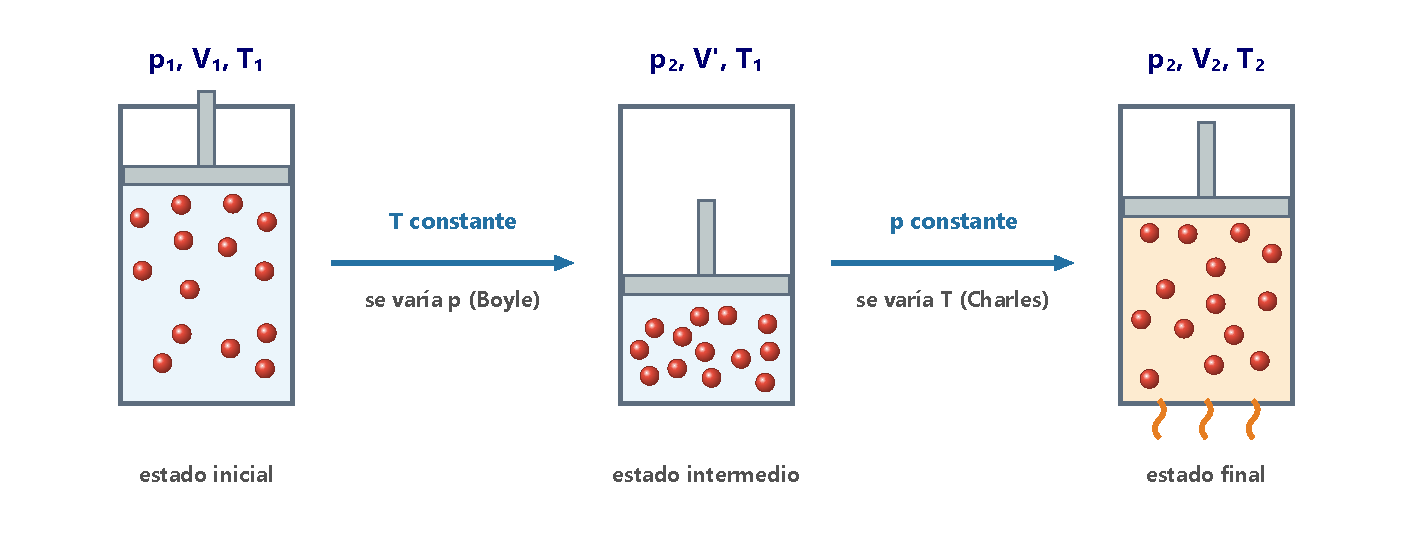
\includegraphics[width=0.8\textwidth]{images/UD1/ley_combinada}
    \caption{Deducción de la ley combinada en dos pasos: primero a \(T\) constante y después a \(p\) constante.}
    \label{fig:ud1-ley-combinada}
\end{figure}

\begin{example}
    \textbf{Calentar un gas.} Un recipiente contiene \qty{4}{\litre} de cloro a \qty{25}{\degreeCelsius} y \qty{750}{\mmHg}. Se
    calienta hasta \qty{50}{\degreeCelsius} y la presión final es de \qty{2}{\atm}. ¿Cuál es el volumen final?

    \textbf{Solución.} Datos: \(p_1 = 750 \cdot \dfrac{1}{760} = \qty{0.987}{\atm}\), \(V_1 = \qty{4}{\litre}\),
    \(T_1 = 25 + 273 = \qty{298}{\kelvin}\); \(p_2 = \qty{2}{\atm}\), \(T_2 = \qty{323}{\kelvin}\).
    \[ \frac{p_1 V_1}{T_1} = \frac{p_2 V_2}{T_2} \Rightarrow V_2 = \frac{p_1 V_1 T_2}{T_1 p_2} =
    \frac{\num{0.987} \cdot 4 \cdot 323}{298 \cdot 2} = \qty{2.14}{\litre} \]
\end{example}

\begin{exercise}
    Un gas ocupa \qty{600}{\milli\litre} a \qty{740}{\mmHg} y \qty{20}{\degreeCelsius}. Si se expande hasta
    \qty{1000}{\milli\litre} y su temperatura sube a \qty{35}{\degreeCelsius}, ¿cuál será su presión?
    \begin{solu}
        \(p_2 = \dfrac{p_1 V_1 T_2}{T_1 V_2} = \dfrac{740 \cdot 600 \cdot 308}{293 \cdot 1000} = \qty{466.7}{\mmHg} =
        \textcolor{red}{\qty{0.614}{\atm}}\).
    \end{solu}
\end{exercise}

%========================================================================================
\section{Teoría cinético-molecular de los gases}\label{sec:ud1-tcm}
%========================================================================================

Las leyes de los gases dicen \emph{cómo} se comportan; la \textbf{teoría cinético-molecular} explica \emph{por qué}. Es un
\textbf{modelo} desarrollado en el siglo \textsc{xix} por \textbf{Joule}, \textbf{Clausius}, \textbf{Maxwell} y
\textbf{Boltzmann}, entre otros.

\begin{definition}[Postulados de la teoría cinético-molecular de los gases]
    \leavevmode % el título de la definición en su propia línea, la lista debajo
    \begin{enumerate}[label=\numberballblue]
        \item Los gases están formados por partículas (átomos o moléculas) de tamaño despreciable frente a las distancias que
        las separan: se pueden considerar \textbf{puntuales}.
        \item Las partículas se mueven continuamente, en línea recta y al \textbf{azar}, chocando entre sí y con las paredes del
        recipiente. Los choques contra las paredes producen la \textbf{presión} del gas.
        \item Los choques son \textbf{elásticos}: no se pierde energía, solo se transfiere de unas partículas a otras.
        \item Las fuerzas de atracción y repulsión entre las partículas son \textbf{despreciables}.
        \item La \textbf{energía cinética media} de las partículas es directamente proporcional a la \textbf{temperatura
        absoluta}: \(\overline{E_c} = k \cdot T\).
    \end{enumerate}
\end{definition}

\subsection{La teoría cinético-molecular explica las leyes de los gases}

\begin{itemize}
    \item \textbf{Boyle-Mariotte.} Si la temperatura no cambia, la velocidad media de las partículas tampoco. Al reducir el
    volumen, tienen menos espacio y chocan con más frecuencia contra las paredes: la presión aumenta.
    \item \textbf{Gay-Lussac.} Si el volumen es fijo y la temperatura sube, las partículas se mueven más deprisa: chocan más a
    menudo y con más fuerza contra las paredes, y la presión aumenta.
    \item \textbf{Charles.} En un recipiente con un émbolo que se mueve libremente, al subir la temperatura los choques más
    frecuentes e intensos empujan el émbolo hacia arriba; el volumen aumenta hasta que la presión interior vuelve a igualar a
    la exterior.
\end{itemize}

\begin{figure}[H]
    \centering
    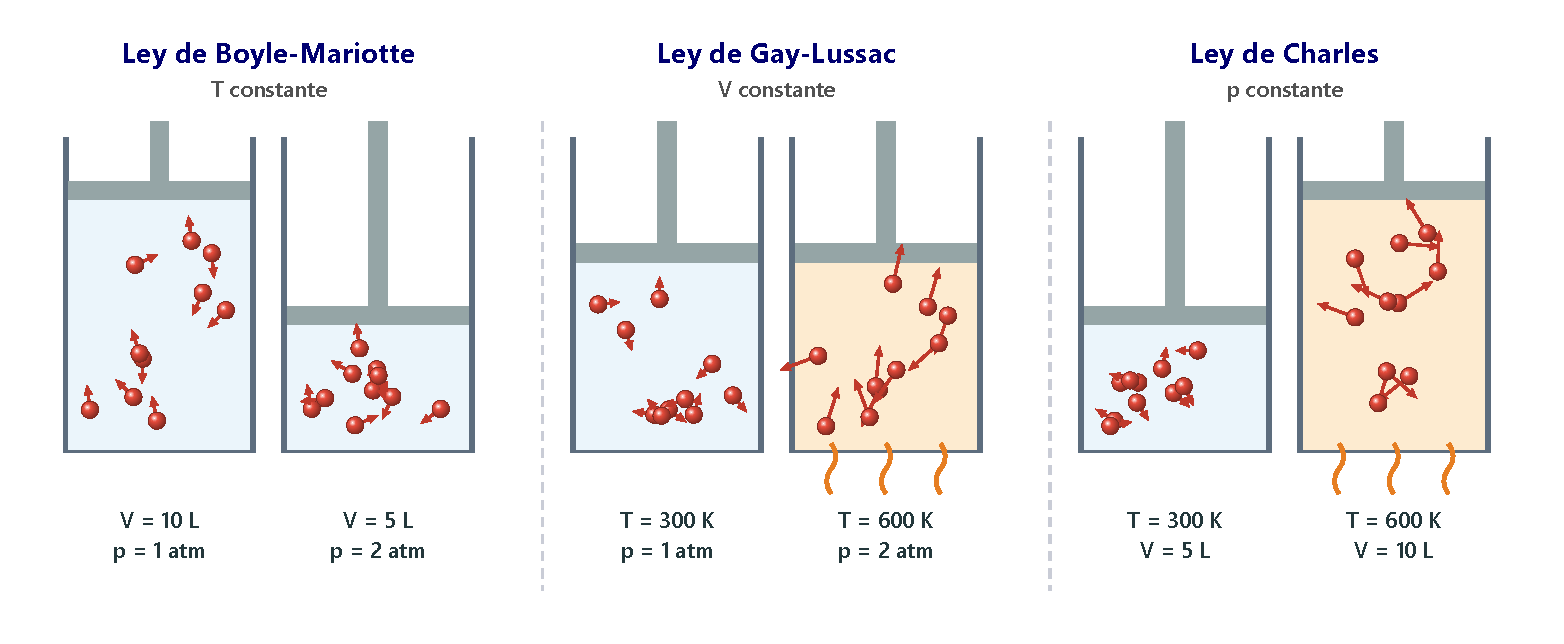
\includegraphics[width=\textwidth]{images/UD1/tcm_leyes}
    \caption{Interpretación cinético-molecular de las leyes de Boyle-Mariotte, Gay-Lussac y Charles. Las flechas indican la
    velocidad de las partículas.}
    \label{fig:ud1-tcm}
\end{figure}

\begin{example}
    \textbf{Temperatura y energía cinética.} ¿Cómo varía la energía cinética de las partículas de un gas si se duplica su
    temperatura absoluta?

    \textbf{Solución.} Según el quinto postulado, \(\overline{E_c} = k\,T\): si \(T\) se duplica, la energía cinética media de
    las partículas también se duplica. Las partículas se mueven más deprisa (su velocidad media aumenta, aunque no al doble,
    porque \(E_c\) depende de \(v^2\)).
\end{example}

%========================================================================================
\section{Ecuación de estado de los gases ideales}\label{sec:ud1-gases-ideales}
%========================================================================================

Un \textbf{gas ideal} es el que cumple exactamente los postulados de la teoría cinético-molecular y, por tanto, las leyes de los
gases. No existe, pero a presiones bajas y temperaturas no muy bajas los gases reales se comportan casi como ideales.

Por la ley de Avogadro, el volumen de un gas a \(p\) y \(T\) dadas es proporcional al número de partículas, es decir, al número
de moles. Por tanto, la constante de la ley combinada, \(p V / T\), es proporcional a \(n\): \(\dfrac{p V}{T} = n R\).

\begin{definition}[Ecuación de estado de los gases ideales]
    \[ p \cdot V = n \cdot R \cdot T \]
    \(R\) es la \textbf{constante de los gases ideales}. Su valor depende de las unidades:
    \(R = \qty{0.082}{\atm\litre\per\mole\per\kelvin}\) (presión en atm y volumen en L) o
    \(R = \qty{8.31}{\pascal\cubic\metre\per\mole\per\kelvin} = \qty{8.31}{\joule\per\mole\per\kelvin}\) (unidades del SI).
\end{definition}

\begin{example}
    \textbf{Valor de \(R\).} Comprueba que \(R\) vale aproximadamente \qty{0.082}{\atm\litre\per\mole\per\kelvin} sabiendo que
    \qty{640}{\gram} de oxígeno, \ch{O2}, a una presión de \qty{4e5}{\pascal}, ocupan \qty{50}{\litre} a \qty{120}{\kelvin}.

    \textbf{Solución.} \(n = \dfrac{640}{32} = \qty{20}{\mole}\); \(p = \dfrac{\num{4e5}}{\num{1.013e5}} = \qty{3.95}{\atm}\).
    \[ R = \frac{p V}{n T} = \frac{\num{3.95} \cdot 50}{20 \cdot 120} = \qty{0.082}{\atm\litre\per\mole\per\kelvin} \]
    El valor coincide con el tabulado: en estas condiciones el oxígeno se comporta como un gas ideal.
\end{example}

\begin{exercise}
    Calcula la presión que ejercen \qty{60}{\gram} de cloro, \ch{Cl2}, en un recipiente de \qty{4}{\cubic\deci\metre} a
    \qty{25}{\degreeCelsius}.
    \begin{solu}
        \(n = 60/71 = \qty{0.845}{\mole}\); \(p = \dfrac{n R T}{V} = \dfrac{\num{0.845} \cdot \num{0.082} \cdot 298}{4} =
        \textcolor{red}{\qty{5.16}{\atm}}\).
    \end{solu}
\end{exercise}

\begin{exercise}
    ¿Qué volumen ocupan \qty{2.5}{\mole} de un gas en condiciones normales (\qty{1}{\atm} y \qty{273}{\kelvin})?
    \begin{solu}
        \(V = \dfrac{n R T}{p} = \num{2.5} \cdot \num{0.082} \cdot 273 = \textcolor{red}{\qty{56}{\litre}}\) \textcolor{blue}{(\(\num{2.5} \cdot \num{22.4}\)).}
    \end{solu}
\end{exercise}

\begin{exercise}
    ¿A qué temperatura deben estar \qty{40}{\gram} de nitrógeno, \ch{N2}, en un recipiente de \qty{400}{\cubic\centi\metre} para
    que su presión sea de \qty{4e6}{\pascal}?
    \begin{solu}
        \(n = 40/28 = \qty{1.43}{\mole}\); \(p = \num{4e6}/\num{1.013e5} = \qty{39.5}{\atm}\);
        \(T = \dfrac{p V}{n R} = \dfrac{\num{39.5} \cdot \num{0.4}}{\num{1.43} \cdot \num{0.082}} = \textcolor{red}{\qty{135}{\kelvin}}\).
    \end{solu}
\end{exercise}

\begin{exercise}
    ¿Qué masa de dióxido de carbono hay en un depósito de \qty{250}{\cubic\metre} en condiciones estándar
    (\qty{1e5}{\pascal} y \qty{273}{\kelvin})?
    \begin{solu}
        \textcolor{blue}{En el SI:} \(n = \dfrac{p V}{R T} = \dfrac{\num{1e5} \cdot 250}{\num{8.31} \cdot 273} = \qty{11020}{\mole}\);
        \(m = \num{11020} \cdot 44 = \qty{4.85e5}{\gram} = \textcolor{red}{\qty{485}{\kilogram}}\).
    \end{solu}
\end{exercise}

\subsection{Volumen molar}

Según la ley de Avogadro, el volumen de un gas no depende de su naturaleza, sino del número de partículas. Se llama
\textbf{volumen molar} al volumen que ocupa un mol de cualquier gas en unas condiciones determinadas. Suelen usarse dos
referencias:
\begin{itemize}
    \item \textbf{Condiciones normales} (c.\,n.): \(p = \qty{1}{\atm}\) y \(T = \qty{273}{\kelvin}\):
    \(V_m = \dfrac{1 \cdot \num{0.082} \cdot 273}{1} = \qty{22.4}{\litre\per\mole}\).
    \item \textbf{Condiciones estándar} de la IUPAC: \(p = \qty{1e5}{\pascal}\) y \(T = \qty{273}{\kelvin}\):
    \(V_m = \qty{22.7}{\litre\per\mole}\).
\end{itemize}

\begin{example}
    \textbf{Volumen de un gas.} Calcula el volumen que ocupan \qty{210}{\gram} de nitrógeno, \ch{N2}, en condiciones estándar.

    \textbf{Solución.} \(\qty{210}{\gram} \cdot \dfrac{\qty{1}{\mole}}{\qty{28}{\gram}} = \qty{7.5}{\mole}\);
    \(\qty{7.5}{\mole} \cdot \dfrac{\qty{22.7}{\litre}}{\qty{1}{\mole}} = \qty{170}{\litre}\).
\end{example}

\subsection{Densidad de un gas}

La densidad de un líquido o de un sólido apenas cambia con las condiciones, pero la de un gas varía mucho con la presión y la
temperatura. Sustituyendo \(n = m/M\) en la ecuación de los gases:
\[ p V = \frac{m}{M} R T \;\Rightarrow\; p = \frac{m}{V} \cdot \frac{R T}{M} = d \cdot \frac{R T}{M} \;\Rightarrow\;
\boxed{d = \frac{p \cdot M}{R \cdot T}} \]
A la misma presión y temperatura, es más denso el gas de \textbf{mayor masa molar}.

\subsection{Masa molar de un gas}

Si no conocemos la fórmula de una sustancia gaseosa, podemos determinar su masa molar en el laboratorio midiendo el volumen
que ocupa una masa conocida a una presión y una temperatura dadas:
\[ p V = \frac{m}{M} R T \;\Rightarrow\; M = \frac{m \cdot R \cdot T}{p \cdot V} \]
Con la masa molar y la fórmula empírica se obtiene la fórmula molecular (apartado~\ref{sec:ud1-formula}).

\begin{example}
    \textbf{Masa molar de un gas.} \qty{45}{\milli\gram} de un gas ocupan \qty{6}{\cubic\centi\metre} en condiciones normales.
    Calcula su masa molar.

    \textbf{Solución.} Pasamos a las unidades de \(R\): \(m = \qty{0.045}{\gram}\), \(V = \qty{0.006}{\litre}\).
    \[ M = \frac{m R T}{p V} = \frac{\num{0.045} \cdot \num{0.082} \cdot 273}{1 \cdot \num{0.006}} = \qty{168}{\gram\per\mole} \]
\end{example}

\subsection{Gases reales}

En condiciones de \textbf{baja presión} y \textbf{alta temperatura}, lejos de los cambios de estado, las partículas están muy
separadas y los gases se comportan casi como ideales. A presiones altas o temperaturas bajas ya no se puede despreciar el
tamaño de las partículas ni las fuerzas entre ellas. En 1873, \textbf{J. D. van der Waals} propuso una ecuación que corrige la
del gas ideal:

\begin{definition}[Ecuación de van der Waals]
    \[ \left(p + \frac{a\,n^2}{V^2}\right)\left(V - n\,b\right) = n R T \]
    La constante \(a\) tiene en cuenta las \textbf{fuerzas de atracción} entre partículas, que reducen la presión; la constante
    \(b\), el \textbf{volumen propio} de las partículas, que reduce el volumen disponible. Ambas son propias de cada gas.
\end{definition}

\begin{remark}
    Si el nitrógeno se comportara como un gas ideal, sus moléculas no se atraerían y nunca se podría licuar. El nitrógeno
    líquido, a \qty{-196}{\degreeCelsius}, se usa en medicina, en la conservación de muestras biológicas y hasta en cocina.
\end{remark}

\begin{example}
    \textbf{Gas real.} Calcula la presión que ejercen \qty{150}{\mole} de aire en un recipiente de \qty{12}{\litre} a
    \qty{30}{\degreeCelsius} con la ecuación de van der Waals (\(a = \qty{1.33}{\atm\litre\squared\per\mole\squared}\),
    \(b = \qty{0.0366}{\litre\per\mole}\)). Compárala con la de un gas ideal.

    \textbf{Solución.} Despejamos la presión:
    \[ p = \frac{n R T}{V - n b} - a \left(\frac{n}{V}\right)^2 = \frac{150 \cdot \num{0.082} \cdot 303}{12 - 150 \cdot \num{0.0366}}
    - \num{1.33} \left(\frac{150}{12}\right)^2 = \num{572.5} - \num{207.8} = \qty{365}{\atm} \]
    Como gas ideal: \(p = \dfrac{150 \cdot \num{0.082} \cdot 303}{12} = \qty{311}{\atm}\). A presiones tan altas la diferencia es
    importante.
\end{example}

\begin{exercise}
    Una sustancia contiene un 24,27\,\% de C, un 4,07\,\% de H y el resto de cloro. \qty{4.00}{\gram} de su vapor ocupan
    \qty{1.24}{\litre} a \qty{100}{\degreeCelsius} y \qty{1}{\atm}. Determina su fórmula molecular.
    \begin{solu}
        \textcolor{blue}{Cl: \qty{71.66}{\percent}.} C \(\num{24.27}/12 = \num{2.02}\); H \(\num{4.07}/1 = \num{4.07}\);
        Cl \(\num{71.66}/\num{35.5} = \num{2.02}\) \(\rightarrow\) 1 : 2 : 1; empírica \ch{CH2Cl}, \(M = \qty{49.5}{\gram\per\mole}\).
        \textcolor{blue}{Masa molar:} \(M = \dfrac{m R T}{p V} = \dfrac{4 \cdot \num{0.082} \cdot 373}{1 \cdot \num{1.24}} = \qty{98.7}{\gram\per\mole}\);
        \(\alpha = \num{98.7}/\num{49.5} = 2\). \textcolor{red}{Fórmula molecular: \ch{C2H4Cl2}}.
    \end{solu}
\end{exercise}

\begin{exercise}
    Calcula la presión ejercida por \qty{4}{\mole} de metanol gaseoso, \ch{CH3OH}, que ocupan \qty{5}{\litre} a \qty{450}{\kelvin}:
    a) suponiendo que es un gas ideal; b) con la ecuación de van der Waals
    (\(a = \qty{9.23}{\atm\litre\squared\per\mole\squared}\), \(b = \qty{0.0651}{\litre\per\mole}\)).
    \begin{solu}
        a) \(p = \dfrac{4 \cdot \num{0.082} \cdot 450}{5} = \textcolor{red}{\qty{29.5}{\atm}}\).
        b) \(p = \dfrac{4 \cdot \num{0.082} \cdot 450}{5 - 4 \cdot \num{0.0651}} - \num{9.23} \left(\dfrac{4}{5}\right)^2 = \num{31.14} - \num{5.91}
        = \textcolor{red}{\qty{25.2}{\atm}}\).
    \end{solu}
\end{exercise}

%========================================================================================
\section{Mezclas de gases}\label{sec:ud1-mezclas}
%========================================================================================

El \textbf{gas natural} que llega a muchas casas es una mezcla: sobre todo metano, con algo de etano, propano, butano,
nitrógeno y dióxido de carbono. El aire también es una mezcla de gases. ¿Cómo se comporta una mezcla?

Se llama \textbf{presión parcial} de un componente, \(p_i\), a la presión que ejercería si estuviera \textbf{él solo} en el
recipiente que ocupa la mezcla, a la misma temperatura. Dalton estudió las mezclas gaseosas y enunció:

\begin{definition}[Ley de Dalton de las presiones parciales]
    La presión total de una mezcla de gases que no reaccionan entre sí es igual a la suma de las presiones parciales de sus
    componentes:
    \[ p_T = p_1 + p_2 + p_3 + \dots = \sum p_i \]
\end{definition}

Cada gas se comporta como si estuviera solo (figura~\ref{fig:ud1-dalton-presiones}). Si en un recipiente de volumen \(V\) y
temperatura \(T\) hay \(n_1\) moles de un gas y \(n_2\) de otro, en total \(n_T = n_1 + n_2\):
\[ p_T = \frac{n_T R T}{V} = \frac{(n_1 + n_2) R T}{V} = \frac{n_1 R T}{V} + \frac{n_2 R T}{V} = p_1 + p_2 \]
Dividiendo la presión parcial de un componente entre la total:
\[ \frac{p_i}{p_T} = \frac{n_i R T / V}{n_T R T / V} = \frac{n_i}{n_T} = \chi_i \]
\(\chi_i\) es la \textbf{fracción molar} del componente: la fracción de las partículas de la mezcla que son de ese gas. Es un
número entre 0 y 1, y la suma de las fracciones molares de todos los componentes vale 1.

\begin{definition}[Presión parcial y fracción molar]
    La presión parcial de un componente de una mezcla de gases es igual a su fracción molar por la presión total:
    \[ p_i = \chi_i \cdot p_T \]
\end{definition}

\begin{figure}[H]
    \centering
    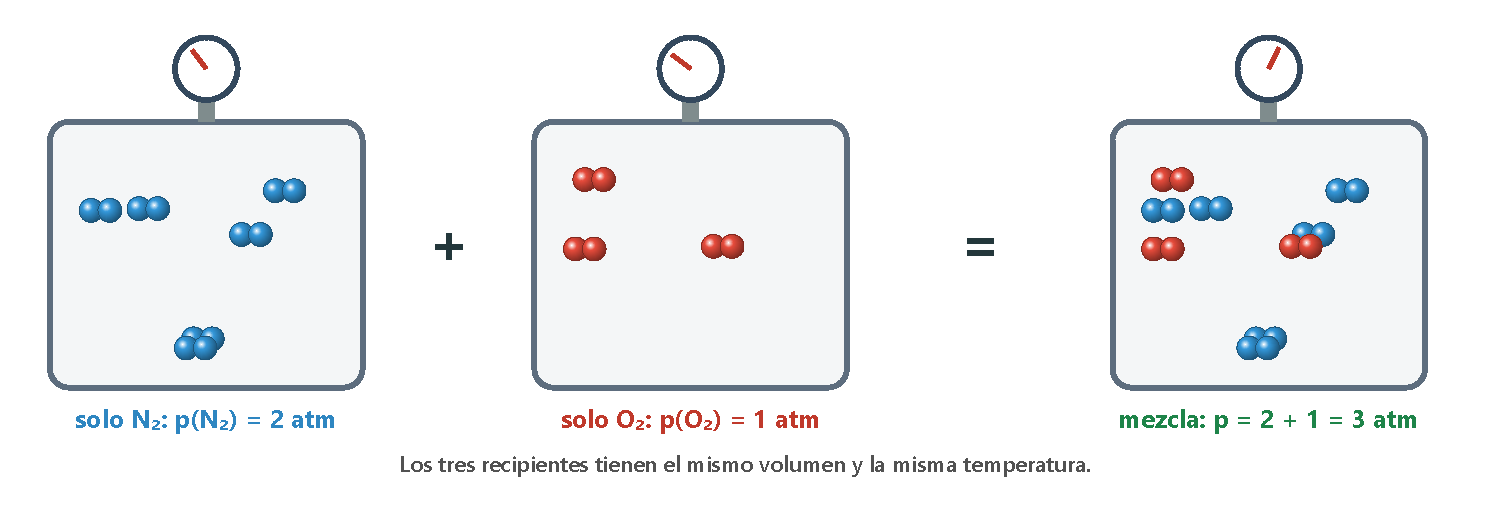
\includegraphics[width=0.85\textwidth]{images/UD1/presiones_parciales}
    \caption{Ley de Dalton: la presión de la mezcla es la suma de las presiones que ejercería cada gas solo.}
    \label{fig:ud1-dalton-presiones}
\end{figure}

\begin{example}
    \textbf{Globo aerostático.} Un globo contiene una mezcla de \qty{70}{\gram} de nitrógeno, \ch{N2}, \qty{32}{\gram} de oxígeno,
    \ch{O2}, y \qty{44}{\gram} de propano, \ch{C3H8}. La presión total es de \qty{4}{\atm}. Calcula la presión parcial de cada
    gas.

    \textbf{Solución.} Moles de cada componente:
    \(n_{\ch{N2}} = \dfrac{70}{28} = \qty{2.5}{\mole}\); \(n_{\ch{O2}} = \dfrac{32}{32} = \qty{1}{\mole}\);
    \(n_{\ch{C3H8}} = \dfrac{44}{44} = \qty{1}{\mole}\); \(n_T = \qty{4.5}{\mole}\).
    \[ p_{\ch{N2}} = \frac{\num{2.5}}{\num{4.5}} \cdot 4 = \qty{2.22}{\atm}; \qquad
       p_{\ch{O2}} = \frac{1}{\num{4.5}} \cdot 4 = \qty{0.89}{\atm}; \qquad
       p_{\ch{C3H8}} = \frac{1}{\num{4.5}} \cdot 4 = \qty{0.89}{\atm} \]
    La suma de las presiones parciales es la presión total: \(\num{2.22} + \num{0.89} + \num{0.89} = \qty{4}{\atm}\).
\end{example}

\begin{exercise}
    Se introducen \qty{120}{\gram} de \ch{CO2} y \qty{140}{\gram} de \ch{CO} en un recipiente de \qty{25}{\litre} a
    \qty{15}{\degreeCelsius}. Calcula: a) la presión total; b) la presión parcial de cada gas.
    \begin{solu}
        a) \(n_{\ch{CO2}} = 120/44 = \qty{2.73}{\mole}\); \(n_{\ch{CO}} = 140/28 = \qty{5}{\mole}\); \(n_T = \qty{7.73}{\mole}\).
        \(p_T = \dfrac{\num{7.73} \cdot \num{0.082} \cdot 288}{25} = \textcolor{red}{\qty{7.30}{\atm}}\).
        b) \(p_{\ch{CO2}} = \dfrac{\num{2.73}}{\num{7.73}} \cdot \num{7.30} = \textcolor{red}{\qty{2.58}{\atm}}\);
        \(p_{\ch{CO}} = \dfrac{5}{\num{7.73}} \cdot \num{7.30} = \textcolor{red}{\qty{4.72}{\atm}}\).
    \end{solu}
\end{exercise}

\begin{exercise}
    Un globo de \qty{6}{\litre} a \qty{25}{\degreeCelsius} contiene helio y hidrógeno con presiones parciales
    \(p(\ch{He}) = \qty{0.6}{\atm}\) y \(p(\ch{H2}) = \qty{0.8}{\atm}\). Calcula: a) la presión total; b) los moles totales;
    c) los moles de cada gas.
    \begin{solu}
        a) \(p_T = \num{0.6} + \num{0.8} = \textcolor{red}{\qty{1.4}{\atm}}\).
        b) \(n_T = \dfrac{\num{1.4} \cdot 6}{\num{0.082} \cdot 298} = \textcolor{red}{\qty{0.344}{\mole}}\).
        c) \(n_{\ch{He}} = \dfrac{\num{0.6}}{\num{1.4}} \cdot \num{0.344} = \textcolor{red}{\qty{0.147}{\mole}}\);
        \(n_{\ch{H2}} = \textcolor{red}{\qty{0.196}{\mole}}\).
    \end{solu}
\end{exercise}

\begin{exercise}
    El aire tiene, en volumen, un 21\,\% de \ch{O2}, un 78\,\% de \ch{N2} y un 1\,\% de argón. En lo alto de una montaña la
    presión atmosférica es de \qty{0.95}{\atm}. ¿Qué presión ejerce cada gas?
    \begin{solu}
        \textcolor{blue}{En los gases, el porcentaje en volumen coincide con la fracción molar.}
        \(p_{\ch{O2}} = \num{0.21} \cdot \num{0.95} = \textcolor{red}{\qty{0.200}{\atm}}\);
        \(p_{\ch{N2}} = \num{0.78} \cdot \num{0.95} = \textcolor{red}{\qty{0.741}{\atm}}\);
        \(p_{\ch{Ar}} = \num{0.01} \cdot \num{0.95} = \textcolor{red}{\qty{0.0095}{\atm}}\).
    \end{solu}
\end{exercise}

\begin{exercise}
    En una botella de \qty{3}{\litre} a \qty{20}{\degreeCelsius}, la presión debida al oxígeno es de \qty{1200}{\mmHg} y la del
    nitrógeno, de \qty{2800}{\mmHg}. Calcula la masa de cada gas.
    \begin{solu}
        \(p_{\ch{O2}} = 1200/760 = \qty{1.58}{\atm}\): \(n = \dfrac{\num{1.58} \cdot 3}{\num{0.082} \cdot 293} = \qty{0.197}{\mole}\),
        \(m = \textcolor{red}{\qty{6.3}{\gram}}\) de \ch{O2}.
        \(p_{\ch{N2}} = 2800/760 = \qty{3.68}{\atm}\): \(n = \qty{0.460}{\mole}\), \(m = \textcolor{red}{\qty{12.9}{\gram}}\) de \ch{N2}.
    \end{solu}
\end{exercise}

%========================================================================================
\section{Química en la vida: ¿cómo funciona una olla a presión?}\label{sec:ud1-olla}
%========================================================================================

En una olla corriente, el agua no puede pasar de \qty{100}{\degreeCelsius}: a esa temperatura hierve y el calor que le
damos se emplea en evaporarla. En una \textbf{olla a presión} (u olla exprés) la tapa cierra herméticamente. Al calentar, el
vapor no puede escapar y la presión dentro aumenta, igual que en la ley de Gay-Lussac. Y cuanto mayor es la presión, mayor es
la temperatura a la que hierve el agua (figura~\ref{fig:ud1-olla}): con unos \qty{2}{\bar}, el agua hierve a unos
\qty{120}{\degreeCelsius}, y los alimentos se cuecen hasta un 70\,\% más rápido.

\begin{figure}[H]
    \centering
    \begin{tikzpicture}
        \begin{axis}[grafica, width=0.6\linewidth, height=5.2cm,
            xlabel={\(t\) (\unit{\degreeCelsius})}, ylabel={\(p\) (\unit{\atm})},
            xmin=0, xmax=135, ymin=0, ymax=3.2, xtick={0,20,...,140}]
            \addplot[thick, red!75!black, domain=0:132] {10^(8.07131 - 1730.63/(233.426 + x))/760};
            \addplot[dashed, gray] coordinates {(0,1) (100,1) (100,0)};
            \addplot[dashed, gray] coordinates {(0,1.96) (120,1.96) (120,0)};
            \node[font=\scriptsize, anchor=south east] at (axis cs:98,1) {olla abierta};
            \node[font=\scriptsize, anchor=south east] at (axis cs:118,1.96) {olla a presión};
        \end{axis}
    \end{tikzpicture}
    \caption{Presión a la que hierve el agua en función de la temperatura (presión de vapor del agua).}
    \label{fig:ud1-olla}
\end{figure}

Cuando se alcanza la presión máxima, una \textbf{válvula} (con un muelle o un contrapeso) se abre y deja salir vapor, de modo
que la presión ya no sube más. Desde ese momento no sirve de nada mantener el fuego fuerte: basta con un fuego bajo que
mantenga la presión, y así se ahorra energía. El silbido característico de algunas ollas lo produce el vapor al salir por el
pequeño orificio de la válvula.

\begin{exercise}
    a) ¿Qué ley de los gases explica que la presión aumente al calentar la olla cerrada? b) ¿Por qué se cocinan antes los
    alimentos en una olla a presión? c) ¿Por qué no conviene abrir la olla nada más apagar el fuego?
    \begin{solu}
        a) \textcolor{red}{La ley de Gay-Lussac}: a volumen constante, la presión es proporcional a la temperatura absoluta (además, al
        evaporarse agua aumenta la cantidad de gas). b) \textcolor{red}{Porque a mayor presión el agua hierve a mayor temperatura}
        (unos \qty{120}{\degreeCelsius} a \qty{2}{\bar}), y las reacciones de la cocción son más rápidas. c) \textcolor{red}{Porque dentro
        la presión sigue siendo alta}: al abrirla, el vapor y el agua muy caliente saldrían con violencia. Hay que esperar a que se
        enfríe o liberar el vapor por la válvula.
    \end{solu}
\end{exercise}

%========================================================================================
\section{Prácticas: química en la cocina}\label{sec:ud1-practicas}
%========================================================================================

\subsection{La ley de Boyle-Mariotte con una nube}

\begin{multicols}{2}
    \textbf{Objetivo}
    \begin{itemize}
        \item Comprobar en casa la ley de Boyle-Mariotte.
    \end{itemize}
    \columnbreak
    \textbf{Material}
    \begin{itemize}
        \item Una jeringuilla grande (de 20 a \qty{50}{\milli\litre}) sin aguja.
        \item Nubes de golosina o un trozo de esponja de baño.
        \item Cinta adhesiva.
    \end{itemize}
\end{multicols}

\textbf{Procedimiento}
\begin{enumerate}[label=\numberballgreen]
    \item \textbf{Parte 1.} Saca el émbolo, mete una nube en la jeringuilla (recórtala si no cabe) y vuelve a colocar el émbolo
    hasta que casi toque la nube. Tapa bien la boquilla con cinta adhesiva.
    \item Tira del émbolo hacia fuera todo lo que puedas y observa la nube. Después vuelve a empujarlo hasta la posición
    inicial (figura~\ref{fig:ud1-practica-boyle}).
    \item \textbf{Parte 2.} Destapa la boquilla, empuja el émbolo hasta que toque la nube y vuelve a taparla. Ahora empuja el
    émbolo: la nube se encoge. Al soltarlo, vuelve a su estado inicial.
\end{enumerate}

\begin{figure}[H]
    \centering
    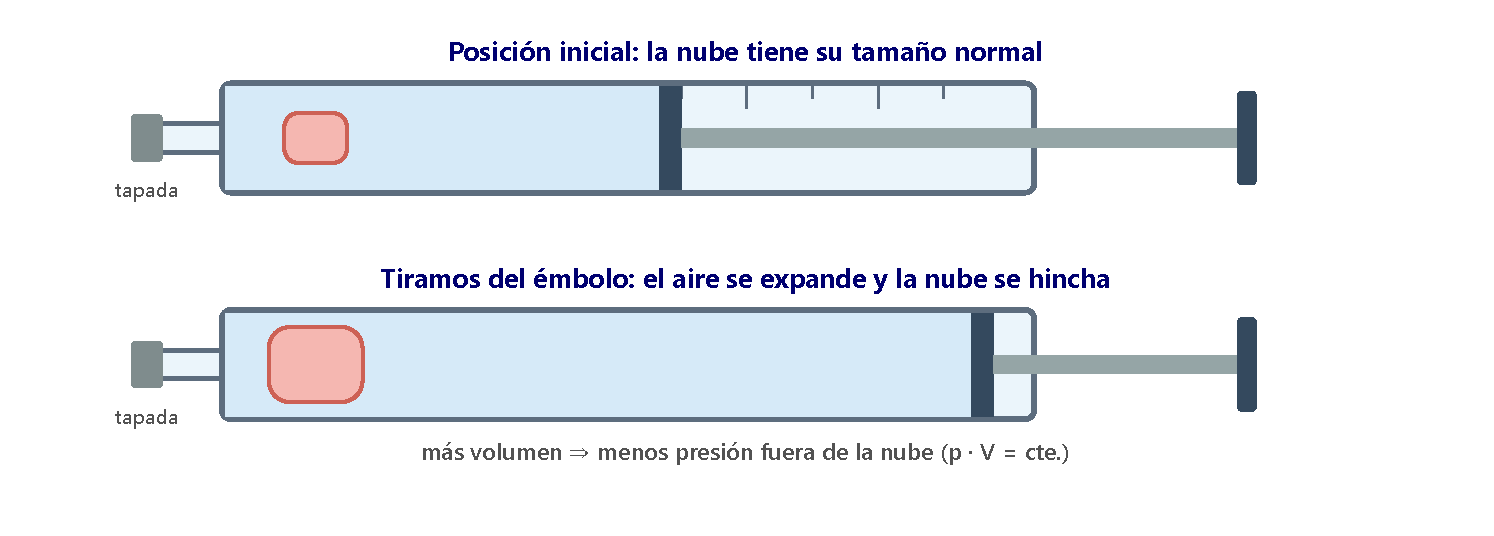
\includegraphics[width=0.85\textwidth]{images/UD1/practica_boyle}
    \caption{Al tirar del émbolo con la boquilla tapada, el aire de la jeringuilla se expande, su presión baja y la nube se
    hincha.}
    \label{fig:ud1-practica-boyle}
\end{figure}

\begin{exercise}
    a) Explica qué le sucede a la nube en cada parte del experimento. b) Utiliza la ley de Boyle-Mariotte para justificarlo.
    \begin{solu}
        a) \textcolor{red}{Al tirar del émbolo la nube se hincha mucho; al empujarlo, se encoge}; en ambos casos recupera su tamaño al
        volver a la posición inicial. b) \textcolor{blue}{La nube está llena de burbujas de aire. Al tirar del émbolo aumenta el volumen
        de la jeringuilla y, como \(p V\) es constante a temperatura constante, la presión del aire que rodea la nube baja.} El
        aire de las burbujas, a más presión que el de fuera, se expande hasta igualar presiones: \textcolor{red}{la nube crece}. Al
        empujar el émbolo ocurre lo contrario: sube la presión y el aire de las burbujas se comprime.
    \end{solu}
\end{exercise}

\subsection{¿Qué tienen que ver los tsunamis con los gases?}

\begin{multicols}{2}
    \textbf{Objetivo}
    \begin{itemize}
        \item Observar cómo un cambio de temperatura de un gas produce un cambio de presión capaz de mover agua.
    \end{itemize}
    \columnbreak
    \textbf{Material y reactivos}
    \begin{itemize}
        \item Plato hondo, vaso de vidrio estrecho, mechero de cocina.
        \item Alcohol de 70°, colorante alimentario y agua.
    \end{itemize}
\end{multicols}

\textbf{Procedimiento}
\begin{enumerate}[label=\numberballgreen]
    \item Echa agua en el plato hasta cubrir dos dedos de profundidad, añade dos gotas de colorante y remueve.
    \item Humedece con un poco de alcohol el interior del vaso y enciéndelo con el mechero. \textbf{Hazlo con un adulto y lejos de
    materiales que puedan arder.}
    \item Coloca enseguida el vaso boca abajo en el plato y observa lo que sucede (puedes grabarlo en vídeo y verlo a cámara
    lenta).
\end{enumerate}

\begin{exercise}
    a) Describe lo que ocurre. b) Explica, con las leyes de los gases, por qué sube el agua dentro del vaso.
    c) Busca información: ¿cómo se forman los tsunamis reales? ¿Tendría sentido un sistema de alerta de tsunamis en España?
    \begin{solu}
        a) \textcolor{red}{La llama se apaga y el agua del plato entra con rapidez en el vaso}, formando una «ola» en el plato.
        b) \textcolor{blue}{La combustión calienta el aire del vaso. Al apagarse la llama, el gas se enfría a volumen casi constante y,
        por la ley de Gay-Lussac, su presión baja} (además, parte del vapor de agua formado se condensa). \textcolor{red}{La presión
        atmosférica, mayor que la del interior, empuja el agua hacia dentro} hasta igualar presiones.
        c) \textcolor{red}{Los tsunamis se producen sobre todo por terremotos submarinos} que desplazan bruscamente grandes masas de agua;
        también por erupciones o deslizamientos. Sí tiene sentido: el golfo de Cádiz y el Mediterráneo han sufrido tsunamis
        (como el que siguió al terremoto de Lisboa de 1755), y España cuenta con un sistema de alerta.
    \end{solu}
\end{exercise}

%========================================================================================
\section{Situación de aprendizaje: mujeres y ciencia (ODS 5)}\label{sec:ud1-ods}
%========================================================================================

El \textbf{Objetivo de Desarrollo Sostenible 5} busca la \textbf{igualdad de género}: que mujeres y niñas tengan los mismos
derechos y oportunidades que los hombres y vivan libres de violencia. La Declaración Universal de los Derechos Humanos de 1948
ya afirmaba que todos los seres humanos nacen libres e iguales en dignidad y derechos. Sin embargo, todavía hay países sin
leyes que protejan la igualdad, y en la ciencia la desigualdad sigue siendo visible: hasta 2023, menos de 30 mujeres habían
recibido un premio Nobel de Física, Química o Medicina, frente a varios cientos de hombres, y en el mundo menos del 30\,\% de
las personas que investigan son mujeres.

\begin{marker}
    \textbf{Reto:} analizad la presencia de las mujeres en la ciencia y proponed medidas para reducir la brecha de género en
    las materias científicas de vuestro centro.
\end{marker}

\begin{enumerate}[label=\numberballred]
    \item \textbf{Veo, pienso, me pregunto.} Buscad titulares recientes sobre mujeres y ciencia (premios Nobel, puestos de
    dirección en investigación, porcentaje de investigadoras). De forma individual, anotad qué veis, qué pensáis y qué preguntas
    os surgen.
    \item \textbf{Investigación.} Elegid a una de las mujeres premiadas con el Nobel de Química o de Física (Marie Curie,
    Irène Joliot-Curie, Dorothy Crowfoot Hodgkin, Ada Yonath, Frances Arnold, Emmanuelle Charpentier, Jennifer Doudna,
    Donna Strickland, Andrea Ghez, Anne L'Huillier…). ¿Por qué recibió el premio? ¿Qué dificultades encontró?
    \item \textbf{Análisis.} ¿Qué opináis de que tan pocos premios científicos hayan sido para mujeres? ¿Cuál creéis que es
    el motivo principal? ¿Ocurre lo mismo en todas las disciplinas?
    \item \textbf{Propuesta.} Redactad un plan de medidas concretas para que en vuestro centro haya un porcentaje igualitario de
    chicas y chicos en las materias científicas, y presentadlo al resto de la clase.
\end{enumerate}
